\documentclass[./main.tex]{subfiles} 
\begin{document}

\subsection{Adaptive AR Model Based Time-Frequency Estimation}

\subsubsection{Stationary Estimation}

Using the Yule Walker eqations and the \texttt{MATLAB} function \texttt{aryule}, we can try and estimate an AR(1) model. This clearly will be difficult, since the signal is non stationary. Thus the model for the first part of the signal will likely not be valid for the second part of the signal etc. Figure \ref{fig:4_2_a} does show the AR(1) attempt to fit to the signal, but it will likely fail across the entire time of the signal (as it goes through different stationary outputs).

\begin{figure}[h]
	\centering 
	\resizebox{\textwidth}{!}{% This file was created by matlab2tikz v0.4.7 (commit dc5325fc96215cb6277fcef9395ab1c97c9c1938) running on MATLAB 8.3.
% Copyright (c) 2008--2014, Nico Schlömer <nico.schloemer@gmail.com>
% All rights reserved.
% Minimal pgfplots version: 1.3
% 
% The latest updates can be retrieved from
%   http://www.mathworks.com/matlabcentral/fileexchange/22022-matlab2tikz
% where you can also make suggestions and rate matlab2tikz.
% 
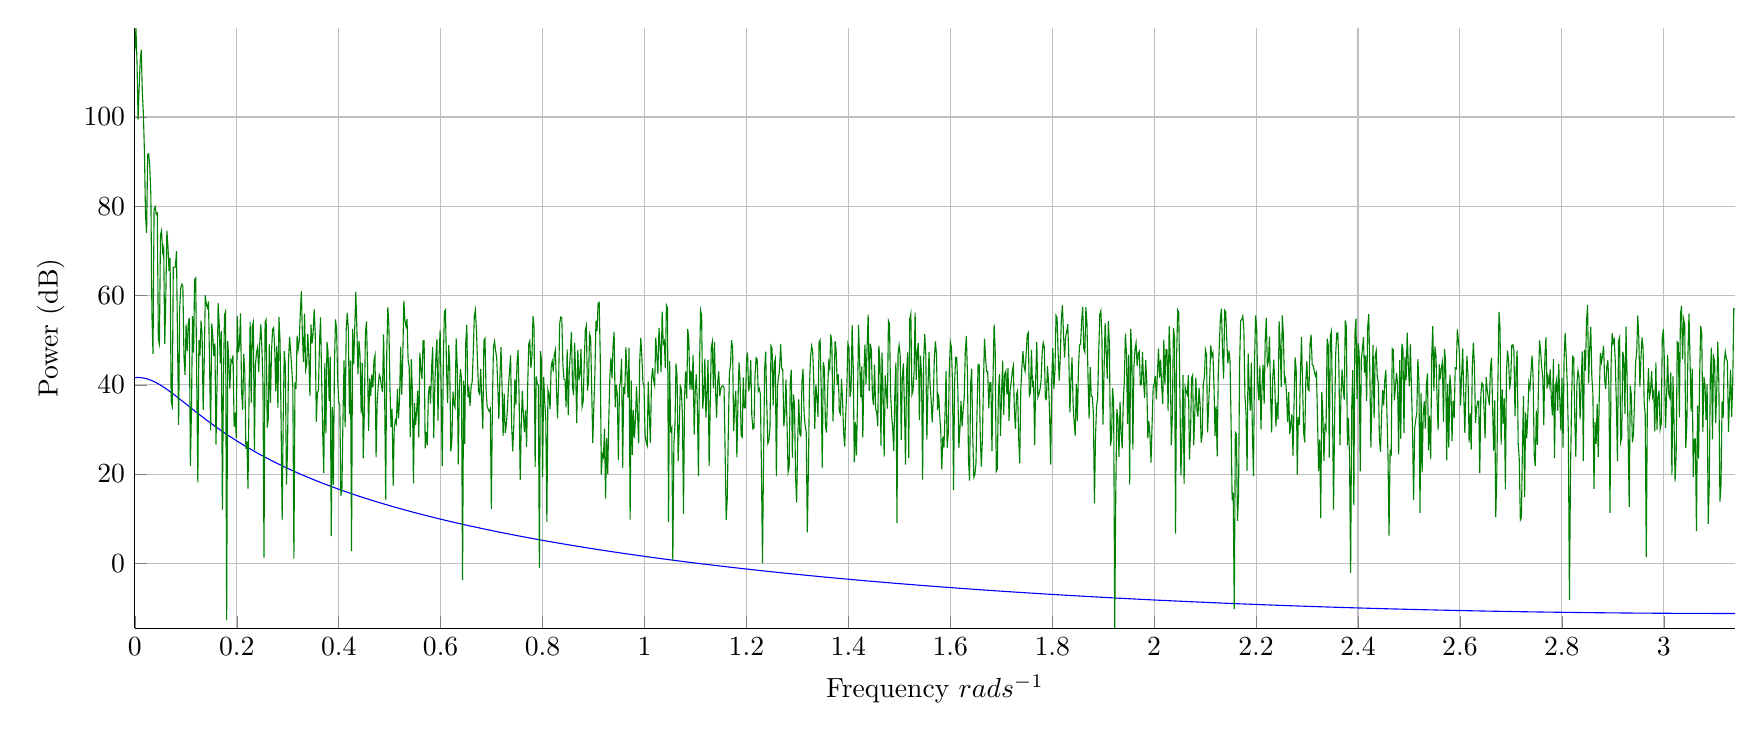
\begin{tikzpicture}

\begin{axis}[%
width=8in,
height=3in,
scale only axis,
xmin=0,
xmax=3.1394982584874,
xlabel={Frequency $rads^{-1}$},
xmajorgrids,
ymin=-14.5376135096419,
ymax=119.898437039073,
ylabel={Power (dB)},
ymajorgrids,
axis x line*=bottom,
axis y line*=left
]
\addplot [color=blue,solid,forget plot]
  table[row sep=crcr]{0	41.603883015879\\
0.0020943951023932	41.6227318598383\\
0.00418879020478639	41.6332582046972\\
0.00628318530717959	41.6354316904032\\
0.00837758040957278	41.6292460375024\\
0.010471975511966	41.6147191074489\\
0.0125663706143592	41.5918927312041\\
0.0146607657167524	41.5608323095719\\
0.0167551608191456	41.5216261932464\\
0.0188495559215388	41.4743848548218\\
0.020943951023932	41.4192398688652\\
0.0230383461263251	41.3563427194773\\
0.0251327412287183	41.2858634574726\\
0.0272271363311115	41.2079892313253\\
0.0293215314335047	41.1229227173317\\
0.0314159265358979	41.030880475023\\
0.0335103216382911	40.9320912537658\\
0.0356047167406843	40.8267942757457\\
0.0376991118430775	40.7152375192391\\
0.0397935069454707	40.5976760243092\\
0.0418879020478639	40.4743702409231\\
0.0439822971502571	40.3455844370743\\
0.0460766922526503	40.2115851819154\\
0.0481710873550435	40.0726399162409\\
0.0502654824574367	39.9290156200141\\
0.0523598775598299	39.7809775840587\\
0.0544542726622231	39.6287882906113\\
0.0565486677646163	39.4727064051962\\
0.0586430628670095	39.3129858802716\\
0.0607374579694027	39.1498751693309\\
0.0628318530717959	38.9836165486376\\
0.0649262481741891	38.8144455425155\\
0.0670206432765823	38.6425904471178\\
0.0691150383789755	38.4682719468304\\
0.0712094334813686	38.2917028169122\\
0.0733038285837618	38.1130877056249\\
0.075398223686155	37.9326229889175\\
0.0774926187885482	37.7504966906989\\
0.0795870138909414	37.5668884618182\\
0.0816814089933346	37.3819696110652\\
0.0837758040957278	37.1959031817726\\
0.085870199198121	37.0088440679333\\
0.0879645943005142	36.8209391641223\\
0.0900589894029074	36.6323275439156\\
0.0921533845053006	36.443140661919\\
0.0942477796076938	36.2535025749468\\
0.096342174710087	36.0635301783088\\
0.0984365698124802	35.8733334535782\\
0.100530964914873	35.6830157246076\\
0.102625360017267	35.4926739189354\\
0.10471975511966	35.3023988320774\\
0.106814150222053	35.1122753925283\\
0.108908545324446	34.9223829255988\\
0.111002940426839	34.7327954144929\\
0.113097335529233	34.5435817572799\\
0.115191730631626	34.3548060186461\\
0.117286125734019	34.1665276755105\\
0.119380520836412	33.9788018557743\\
0.121474915938805	33.7916795696318\\
0.123569311041199	33.6052079330118\\
0.125663706143592	33.4194303828422\\
0.127758101245985	33.234386883937\\
0.129852496348378	33.050114127396\\
0.131946891450771	32.8666457204862\\
0.134041286553165	32.6840123680414\\
0.136135681655558	32.5022420454703\\
0.138230076757951	32.3213601635103\\
0.140324471860344	32.1413897249026\\
0.142418866962737	31.9623514731921\\
0.14451326206513	31.7842640338831\\
0.146607657167524	31.6071440481954\\
0.148702052269917	31.4310062996829\\
0.15079644737231	31.255863833983\\
0.152890842474703	31.0817280719729\\
0.154985237577096	30.9086089166087\\
0.15707963267949	30.7365148537263\\
0.159174027781883	30.5654530470793\\
0.161268422884276	30.3954294278847\\
0.163362817986669	30.2264487791437\\
0.165457213089062	30.0585148149976\\
0.167551608191456	29.8916302553702\\
0.169646003293849	29.7257968961437\\
0.171740398396242	29.5610156751019\\
0.173834793498635	29.3972867338702\\
0.175929188601028	29.2346094760692\\
0.178023583703422	29.0729826218924\\
0.180117978805815	28.9124042593069\\
0.182212373908208	28.7528718920692\\
0.184306769010601	28.5943824847371\\
0.186401164112994	28.4369325048514\\
0.188495559215388	28.2805179624507\\
0.190589954317781	28.1251344470779\\
0.192684349420174	27.9707771624229\\
0.194778744522567	27.8174409587447\\
0.19687313962496	27.6651203632037\\
0.198967534727354	27.5138096082301\\
0.201061929829747	27.3635026580463\\
0.20315632493214	27.2141932334562\\
0.205250720034533	27.0658748350055\\
0.207345115136926	26.9185407646129\\
0.20943951023932	26.7721841457662\\
0.211533905341713	26.6267979423711\\
0.213628300444106	26.4823749763364\\
0.215722695546499	26.3389079439719\\
0.217817090648892	26.1963894312758\\
0.219911485751286	26.0548119281773\\
0.222005880853679	25.9141678418019\\
0.224100275956072	25.7744495088191\\
0.226194671058465	25.635649206931\\
0.228289066160858	25.4977591655543\\
0.230383461263251	25.3607715757486\\
0.232477856365645	25.2246785994355\\
0.234572251468038	25.0894723779569\\
0.236666646570431	24.9551450400105\\
0.238761041672824	24.8216887090055\\
0.240855436775217	24.6890955098728\\
0.242949831877611	24.5573575753657\\
0.245044226980004	24.4264670518831\\
0.247138622082397	24.2964161048467\\
0.24923301718479	24.1671969236589\\
0.251327412287183	24.0388017262702\\
0.253421807389577	23.9112227633807\\
0.25551620249197	23.7844523222985\\
0.257610597594363	23.6584827304784\\
0.259704992696756	23.5333063587612\\
0.261799387799149	23.4089156243326\\
0.263893782901543	23.2853029934205\\
0.265988178003936	23.1624609837488\\
0.268082573106329	23.040382166761\\
0.270176968208722	22.9190591696322\\
0.272271363311115	22.7984846770808\\
0.274365758413509	22.6786514329942\\
0.276460153515902	22.5595522418823\\
0.278554548618295	22.441179970167\\
0.280648943720688	22.3235275473232\\
0.282743338823081	22.2065879668765\\
0.284837733925475	22.0903542872723\\
0.286932129027868	21.9748196326208\\
0.289026524130261	21.8599771933296\\
0.291120919232654	21.74582022663\\
0.293215314335047	21.6323420570049\\
0.295309709437441	21.5195360765257\\
0.297404104539834	21.4073957451036\\
0.299498499642227	21.2959145906631\\
0.30159289474462	21.1850862092415\\
0.303687289847013	21.0749042650209\\
0.305781684949407	20.9653624902981\\
0.3078760800518	20.8564546853957\\
0.309970475154193	20.7481747185197\\
0.312064870256586	20.6405165255682\\
0.314159265358979	20.5334741098937\\
0.316253660461373	20.4270415420241\\
0.318348055563766	20.3212129593444\\
0.320442450666159	20.2159825657434\\
0.322536845768552	20.1113446312275\\
0.324631240870945	20.0072934915056\\
0.326725635973338	19.9038235475455\\
0.328820031075732	19.8009292651069\\
0.330914426178125	19.698605174251\\
0.333008821280518	19.5968458688307\\
0.335103216382911	19.4956460059613\\
0.337197611485304	19.3950003054759\\
0.339292006587698	19.2949035493653\\
0.341386401690091	19.1953505812047\\
0.343480796792484	19.0963363055695\\
0.345575191894877	18.9978556874397\\
0.34766958699727	18.899903751597\\
0.349763982099664	18.8024755820122\\
0.351858377202057	18.7055663212278\\
0.35395277230445	18.6091711697344\\
0.356047167406843	18.5132853853419\\
0.358141562509236	18.4179042825489\\
0.36023595761163	18.3230232319073\\
0.362330352714023	18.2286376593863\\
0.364424747816416	18.134743045735\\
0.366519142918809	18.041334925844\\
0.368613538021202	17.9484088881073\\
0.370707933123596	17.8559605737857\\
0.372802328225989	17.7639856763698\\
0.374896723328382	17.6724799409464\\
0.376991118430775	17.5814391635659\\
0.379085513533168	17.4908591906133\\
0.381179908635562	17.4007359181812\\
0.383274303737955	17.3110652914472\\
0.385368698840348	17.221843304054\\
0.387463093942741	17.1330659974947\\
0.389557489045134	17.044729460501\\
0.391651884147528	16.9568298284373\\
0.393746279249921	16.8693632826986\\
0.395840674352314	16.7823260501137\\
0.397935069454707	16.6957144023538\\
0.4000294645571	16.609524655346\\
0.402123859659494	16.5237531686927\\
0.404218254761887	16.4383963450963\\
0.40631264986428	16.3534506297897\\
0.408407044966673	16.268912509973\\
0.410501440069066	16.1847785142556\\
0.41259583517146	16.1010452121045\\
0.414690230273853	16.0177092132991\\
0.416784625376246	15.9347671673915\\
0.418879020478639	15.8522157631733\\
0.420973415581032	15.7700517281487\\
0.423067810683426	15.6882718280137\\
0.425162205785819	15.6068728661416\\
0.427256600888212	15.5258516830751\\
0.429350995990605	15.4452051560239\\
0.431445391092998	15.3649301983695\\
0.433539786195391	15.2850237591758\\
0.435634181297785	15.205482822706\\
0.437728576400178	15.1263044079459\\
0.439822971502571	15.0474855681332\\
0.441917366604964	14.9690233902933\\
0.444011761707357	14.8909149947812\\
0.446106156809751	14.8131575348293\\
0.448200551912144	14.7357481961015\\
0.450294947014537	14.6586841962535\\
0.45238934211693	14.581962784499\\
0.454483737219323	14.5055812411813\\
0.456578132321717	14.4295368773523\\
0.45867252742411	14.3538270343556\\
0.460766922526503	14.2784490834166\\
0.462861317628896	14.2034004252382\\
0.464955712731289	14.1286784896018\\
0.467050107833683	14.0542807349742\\
0.469144502936076	13.9802046481201\\
0.471238898038469	13.9064477437204\\
0.473333293140862	13.8330075639954\\
0.475427688243255	13.7598816783336\\
0.477522083345649	13.6870676829265\\
0.479616478448042	13.6145632004076\\
0.481710873550435	13.5423658794975\\
0.483805268652828	13.4704733946537\\
0.485899663755221	13.3988834457258\\
0.487994058857615	13.3275937576153\\
0.490088453960008	13.2566020799409\\
0.492182849062401	13.1859061867084\\
0.494277244164794	13.1155038759853\\
0.496371639267187	13.0453929695807\\
0.498466034369581	12.9755713127293\\
0.500560429471974	12.9060367737802\\
0.502654824574367	12.8367872438908\\
0.50474921967676	12.7678206367248\\
0.506843614779153	12.6991348881542\\
0.508938009881547	12.6307279559667\\
0.51103240498394	12.5625978195765\\
0.513126800086333	12.4947424797403\\
0.515221195188726	12.4271599582765\\
0.517315590291119	12.3598482977892\\
0.519409985393512	12.2928055613962\\
0.521504380495906	12.226029832461\\
0.523598775598299	12.1595192143285\\
0.525693170700692	12.093271830065\\
0.527787565803085	12.0272858222019\\
0.529881960905478	11.961559352483\\
0.531976356007872	11.896090601616\\
0.534070751110265	11.830877769027\\
0.536165146212658	11.7659190726196\\
0.538259541315051	11.7012127485363\\
0.540353936417444	11.6367570509245\\
0.542448331519838	11.5725502517057\\
0.544542726622231	11.5085906403476\\
0.546637121724624	11.4448765236401\\
0.548731516827017	11.3814062254745\\
0.55082591192941	11.3181780866259\\
0.552920307031804	11.2551904645383\\
0.555014702134197	11.1924417331143\\
0.55710909723659	11.1299302825061\\
0.559203492338983	11.0676545189105\\
0.561297887441376	11.0056128643673\\
0.56339228254377	10.9438037565596\\
0.565486677646163	10.8822256486182\\
0.567581072748556	10.8208770089274\\
0.569675467850949	10.7597563209353\\
0.571769862953342	10.6988620829655\\
0.573864258055735	10.6381928080325\\
0.575958653158129	10.5777470236589\\
0.578053048260522	10.5175232716961\\
0.580147443362915	10.4575201081472\\
0.582241838465308	10.3977361029923\\
0.584336233567701	10.3381698400168\\
0.586430628670095	10.2788199166416\\
0.588525023772488	10.2196849437564\\
0.590619418874881	10.1607635455548\\
0.592713813977274	10.1020543593721\\
0.594808209079667	10.0435560355254\\
0.596902604182061	9.98526723715628\\
0.598996999284454	9.92718664007472\\
0.601091394386847	9.86931293260659\\
0.60318578948924	9.81164481544242\\
0.605280184591633	9.75418100148864\\
0.607374579694027	9.69692021572088\\
0.60946897479642	9.63986119503939\\
0.611563369898813	9.58300268812652\\
0.613657765001206	9.52634345530612\\
0.615752160103599	9.4698822684051\\
0.617846555205993	9.41361791061677\\
0.619940950308386	9.35754917636624\\
0.622035345410779	9.30167487117767\\
0.624129740513172	9.24599381154334\\
0.626224135615565	9.19050482479465\\
0.628318530717959	9.13520674897485\\
0.630412925820352	9.08009843271359\\
0.632507320922745	9.02517873510321\\
0.634601716025138	8.97044652557678\\
0.636696111127531	8.91590068378775\\
0.638790506229925	8.8615400994914\\
0.640884901332318	8.80736367242785\\
0.642979296434711	8.7533703122067\\
0.645073691537104	8.69955893819326\\
0.647168086639497	8.64592847939641\\
0.649262481741891	8.5924778743579\\
0.651356876844284	8.53920607104325\\
0.653451271946677	8.48611202673414\\
0.65554566704907	8.43319470792222\\
0.657640062151463	8.38045309020444\\
0.659734457253857	8.32788615817975\\
0.66182885235625	8.27549290534725\\
0.663923247458643	8.2232723340057\\
0.666017642561036	8.17122345515439\\
0.668112037663429	8.11934528839536\\
0.670206432765823	8.06763686183694\\
0.672300827868216	8.01609721199861\\
0.674395222970609	7.96472538371711\\
0.676489618073002	7.9135204300538\\
0.678584013175395	7.86248141220333\\
0.680678408277789	7.81160739940346\\
0.682772803380182	7.76089746884609\\
0.684867198482575	7.71035070558956\\
0.686961593584968	7.65996620247199\\
0.689055988687361	7.60974306002588\\
0.691150383789755	7.55968038639376\\
0.693244778892148	7.50977729724504\\
0.695339173994541	7.46003291569385\\
0.697433569096934	7.41044637221808\\
0.699527964199327	7.36101680457936\\
0.70162235930172	7.31174335774424\\
0.703716754404114	7.26262518380626\\
0.705811149506507	7.2136614419091\\
0.7079055446089	7.16485129817073\\
0.709999939711293	7.11619392560859\\
0.712094334813686	7.06768850406566\\
0.71418872991608	7.0193342201375\\
0.716283125018473	6.97113026710034\\
0.718377520120866	6.92307584483993\\
0.720471915223259	6.87517015978149\\
0.722566310325652	6.82741242482038\\
0.724660705428046	6.7798018592538\\
0.726755100530439	6.73233768871332\\
0.728849495632832	6.68501914509822\\
0.730943890735225	6.63784546650977\\
0.733038285837618	6.59081589718629\\
0.735132680940012	6.54392968743901\\
0.737227076042405	6.49718609358886\\
0.739321471144798	6.45058437790391\\
0.741415866247191	6.4041238085377\\
0.743510261349584	6.35780365946834\\
0.745604656451977	6.3116232104383\\
0.747699051554371	6.26558174689507\\
0.749793446656764	6.21967855993248\\
0.751887841759157	6.17391294623276\\
0.75398223686155	6.12828420800937\\
0.756076631963943	6.0827916529505\\
0.758171027066337	6.03743459416331\\
0.76026542216873	5.99221235011878\\
0.762359817271123	5.94712424459737\\
0.764454212373516	5.90216960663521\\
0.766548607475909	5.8573477704711\\
0.768643002578303	5.81265807549402\\
0.770737397680696	5.7680998661914\\
0.772831792783089	5.72367249209794\\
0.774926187885482	5.67937530774511\\
0.777020582987875	5.63520767261126\\
0.779114978090269	5.59116895107227\\
0.781209373192662	5.54725851235292\\
0.783303768295055	5.50347573047876\\
0.785398163397448	5.45981998422855\\
0.787492558499841	5.41629065708739\\
0.789586953602235	5.37288713720027\\
0.791681348704628	5.32960881732624\\
0.793775743807021	5.28645509479323\\
0.795870138909414	5.24342537145318\\
0.797964534011807	5.20051905363796\\
0.800058929114201	5.15773555211564\\
0.802153324216594	5.11507428204736\\
0.804247719318987	5.07253466294468\\
0.80634211442138	5.03011611862748\\
0.808436509523773	4.98781807718229\\
0.810530904626167	4.94563997092118\\
0.81262529972856	4.90358123634106\\
0.814719694830953	4.8616413140836\\
0.816814089933346	4.81981964889541\\
0.818908485035739	4.77811568958886\\
0.821002880138133	4.73652888900334\\
0.823097275240526	4.69505870396683\\
0.825191670342919	4.6537045952581\\
0.827286065445312	4.61246602756925\\
0.829380460547705	4.5713424694687\\
0.831474855650099	4.53033339336461\\
0.833569250752492	4.48943827546873\\
0.835663645854885	4.44865659576066\\
0.837758040957278	4.40798783795254\\
0.839852436059671	4.36743148945408\\
0.841946831162065	4.32698704133812\\
0.844041226264458	4.28665398830645\\
0.846135621366851	4.24643182865604\\
0.848230016469244	4.20632006424581\\
0.850324411571637	4.16631820046354\\
0.852418806674031	4.12642574619333\\
0.854513201776424	4.08664221378335\\
0.856607596878817	4.04696711901399\\
0.85870199198121	4.00739998106639\\
0.860796387083603	3.96794032249121\\
0.862890782185997	3.92858766917789\\
0.86498517728839	3.8893415503242\\
0.867079572390783	3.8502014984061\\
0.869173967493176	3.81116704914798\\
0.871268362595569	3.77223774149321\\
0.873362757697963	3.73341311757504\\
0.875457152800356	3.69469272268778\\
0.877551547902749	3.65607610525837\\
0.879645943005142	3.61756281681815\\
0.881740338107535	3.57915241197511\\
0.883834733209929	3.54084444838626\\
0.885929128312322	3.50263848673046\\
0.888023523414715	3.46453409068143\\
0.890117918517108	3.42653082688115\\
0.892212313619501	3.38862826491347\\
0.894306708721895	3.35082597727809\\
0.896401103824288	3.31312353936473\\
0.898495498926681	3.27552052942767\\
0.900589894029074	3.23801652856052\\
0.902684289131467	3.20061112067126\\
0.90477868423386	3.16330389245755\\
0.906873079336254	3.12609443338236\\
0.908967474438647	3.08898233564976\\
0.91106186954104	3.05196719418108\\
0.913156264643433	3.01504860659125\\
0.915250659745826	2.97822617316541\\
0.91734505484822	2.94149949683581\\
0.919439449950613	2.90486818315889\\
0.921533845053006	2.86833184029268\\
0.923628240155399	2.83189007897433\\
0.925722635257792	2.79554251249803\\
0.927817030360186	2.75928875669301\\
0.929911425462579	2.7231284299019\\
0.932005820564972	2.68706115295924\\
0.934100215667365	2.65108654917019\\
0.936194610769758	2.61520424428959\\
0.938289005872152	2.57941386650112\\
0.940383400974545	2.54371504639671\\
0.942477796076938	2.50810741695621\\
0.944572191179331	2.4725906135272\\
0.946666586281724	2.43716427380504\\
0.948760981384118	2.40182803781318\\
0.950855376486511	2.36658154788359\\
0.952949771588904	2.33142444863744\\
0.955044166691297	2.29635638696596\\
0.95713856179369	2.26137701201151\\
0.959232956896084	2.22648597514887\\
0.961327351998477	2.19168292996664\\
0.96342174710087	2.15696753224894\\
0.965516142203263	2.12233943995718\\
0.967610537305656	2.08779831321214\\
0.96970493240805	2.05334381427613\\
0.971799327510443	2.01897560753539\\
0.973893722612836	1.98469335948262\\
0.975988117715229	1.95049673869977\\
0.978082512817622	1.91638541584091\\
0.980176907920016	1.88235906361531\\
0.982271303022409	1.84841735677074\\
0.984365698124802	1.81455997207684\\
0.986460093227195	1.78078658830877\\
0.988554488329588	1.74709688623088\\
0.990648883431982	1.71349054858071\\
0.992743278534375	1.67996726005301\\
0.994837673636768	1.64652670728403\\
0.996932068739161	1.61316857883585\\
0.999026463841554	1.579892565181\\
1.00112085894395	1.54669835868707\\
1.00321525404634	1.51358565360166\\
1.00530964914873	1.48055414603733\\
1.00740404425113	1.44760353395673\\
1.00949843935352	1.41473351715797\\
1.01159283445591	1.38194379725996\\
1.01368722955831	1.34923407768811\\
1.0157816246607	1.31660406365994\\
1.01787601976309	1.28405346217103\\
1.01997041486549	1.251581981981\\
1.02206480996788	1.2191893335996\\
1.02415920507027	1.18687522927307\\
1.02625360017267	1.15463938297047\\
1.02834799527506	1.12248151037025\\
1.03044239037745	1.09040132884693\\
1.03253678547985	1.05839855745788\\
1.03463118058224	1.02647291693024\\
1.03672557568463	0.994624129647975\\
1.03881997078702	0.962851919639063\\
1.04091436588942	0.931156012562783\\
1.04300876099181	0.899536135697121\\
1.0451031560942	0.867992017926332\\
1.0471975511966	0.836523389728567\\
1.04929194629899	0.805129983163685\\
1.05138634140138	0.773811531861112\\
1.05348073650378	0.742567771007879\\
1.05557513160617	0.711398437336693\\
1.05766952670856	0.68030326911423\\
1.05976392181096	0.649282006129427\\
1.06185831691335	0.618334389681959\\
1.06395271201574	0.587460162570788\\
1.06604710711814	0.55665906908285\\
1.06814150222053	0.525930854981813\\
1.07023589732292	0.495275267496954\\
1.07233029242532	0.464692055312156\\
1.07442468752771	0.434180968554983\\
1.0765190826301	0.403741758785872\\
1.0786134777325	0.373374178987425\\
1.08070787283489	0.343077983553774\\
1.08280226793728	0.312852928280098\\
1.08489666303968	0.282698770352194\\
1.08699105814207	0.252615268336128\\
1.08908545324446	0.22260218216805\\
1.09117984834685	0.192659273144045\\
1.09327424344925	0.162786303910082\\
1.09536863855164	0.132983038452079\\
1.09746303365403	0.10324924208604\\
1.09955742875643	0.073584681448293\\
1.10165182385882	0.0439891244858112\\
1.10374621896121	0.0144623404466152\\
1.10584061406361	-0.014995900129715\\
1.107935009166	-0.0443858254214692\\
1.11002940426839	-0.0737076623341366\\
1.11212379937079	-0.102961636509649\\
1.11421819447318	-0.132147972335539\\
1.11631258957557	-0.161266892954049\\
1.11840698467797	-0.190318620271083\\
1.12050137978036	-0.219303374965177\\
1.12259577488275	-0.248221376496301\\
1.12469016998515	-0.277072843114625\\
1.12678456508754	-0.305857991869234\\
1.12887896018993	-0.334577038616684\\
1.13097335529233	-0.363230198029553\\
1.13306775039472	-0.3918176836049\\
1.13516214549711	-0.420339707672632\\
1.13725654059951	-0.44879648140381\\
1.1393509357019	-0.477188214818866\\
1.14144533080429	-0.505515116795786\\
1.14353972590668	-0.533777395078185\\
1.14563412100908	-0.561975256283288\\
1.14772851611147	-0.590108905909941\\
1.14982291121386	-0.618178548346411\\
1.15191730631626	-0.646184386878251\\
1.15401170141865	-0.674126623695999\\
1.15610609652104	-0.702005459902859\\
1.15820049162344	-0.729821095522317\\
1.16029488672583	-0.757573729505657\\
1.16238928182822	-0.785263559739444\\
1.16448367693062	-0.812890783052914\\
1.16657807203301	-0.84045559522535\\
1.1686724671354	-0.867958190993329\\
1.1707668622378	-0.895398764057944\\
1.17286125734019	-0.922777507091976\\
1.17495565244258	-0.950094611746957\\
1.17705004754498	-0.977350268660233\\
1.17914444264737	-1.00454466746191\\
1.18123883774976	-1.03167799678178\\
1.18333323285216	-1.05875044425618\\
1.18542762795455	-1.08576219653475\\
1.18752202305694	-1.11271343928722\\
1.18961641815933	-1.13960435721004\\
1.19171081326173	-1.16643513403306\\
1.19380520836412	-1.19320595252603\\
1.19589960346651	-1.21991699450517\\
1.19799399856891	-1.24656844083958\\
1.2000883936713	-1.27316047145767\\
1.20218278877369	-1.29969326535349\\
1.20427718387609	-1.32616700059306\\
1.20637157897848	-1.35258185432054\\
1.20846597408087	-1.37893800276451\\
1.21056036918327	-1.40523562124402\\
1.21265476428566	-1.43147488417474\\
1.21474915938805	-1.45765596507497\\
1.21684355449045	-1.48377903657162\\
1.21893794959284	-1.50984427040615\\
1.22103234469523	-1.53585183744048\\
1.22312673979763	-1.56180190766275\\
1.22522113490002	-1.58769465019324\\
1.22731553000241	-1.61353023328998\\
1.22940992510481	-1.63930882435452\\
1.2315043202072	-1.66503058993755\\
1.23359871530959	-1.6906956957445\\
1.23569311041199	-1.71630430664113\\
1.23778750551438	-1.74185658665897\\
1.23988190061677	-1.76735269900085\\
1.24197629571916	-1.79279280604629\\
1.24407069082156	-1.81817706935686\\
1.24616508592395	-1.84350564968156\\
1.24825948102634	-1.86877870696204\\
1.25035387612874	-1.89399640033792\\
1.25244827123113	-1.91915888815193\\
1.25454266633352	-1.94426632795509\\
1.25663706143592	-1.96931887651186\\
1.25873145653831	-1.99431668980517\\
1.2608258516407	-2.01925992304147\\
1.2629202467431	-2.04414873065576\\
1.26501464184549	-2.0689832663165\\
1.26710903694788	-2.09376368293053\\
1.26920343205028	-2.118490132648\\
1.27129782715267	-2.14316276686713\\
1.27339222225506	-2.16778173623907\\
1.27548661735746	-2.19234719067263\\
1.27758101245985	-2.216859279339\\
1.27967540756224	-2.24131815067648\\
1.28176980266464	-2.26572395239506\\
1.28386419776703	-2.29007683148107\\
1.28595859286942	-2.31437693420177\\
1.28805298797182	-2.33862440610985\\
1.29014738307421	-2.36281939204794\\
1.2922417781766	-2.38696203615313\\
1.29433617327899	-2.41105248186132\\
1.29643056838139	-2.43509087191167\\
1.29852496348378	-2.45907734835096\\
1.30061935858617	-2.4830120525379\\
1.30271375368857	-2.50689512514745\\
1.30480814879096	-2.53072670617502\\
1.30690254389335	-2.55450693494081\\
1.30899693899575	-2.57823595009388\\
1.31109133409814	-2.60191388961641\\
1.31318572920053	-2.62554089082776\\
1.31528012430293	-2.64911709038863\\
1.31737451940532	-2.67264262430507\\
1.31946891450771	-2.69611762793257\\
1.32156330961011	-2.71954223598\\
1.3236577047125	-2.74291658251363\\
1.32575209981489	-2.76624080096109\\
1.32784649491729	-2.78951502411521\\
1.32994089001968	-2.81273938413797\\
1.33203528512207	-2.83591401256432\\
1.33412968022447	-2.859039040306\\
1.33622407532686	-2.88211459765537\\
1.33831847042925	-2.90514081428914\\
1.34041286553165	-2.92811781927208\\
1.34250726063404	-2.95104574106081\\
1.34460165573643	-2.97392470750742\\
1.34669605083882	-2.99675484586312\\
1.34879044594122	-3.01953628278188\\
1.35088484104361	-3.04226914432404\\
1.352979236146	-3.06495355595986\\
1.3550736312484	-3.08758964257306\\
1.35716802635079	-3.11017752846434\\
1.35926242145318	-3.13271733735487\\
1.36135681655558	-3.15520919238978\\
1.36345121165797	-3.17765321614155\\
1.36554560676036	-3.20004953061344\\
1.36764000186276	-3.22239825724291\\
1.36973439696515	-3.24469951690491\\
1.37182879206754	-3.2669534299153\\
1.37392318716994	-3.28916011603407\\
1.37601758227233	-3.31131969446872\\
1.37811197737472	-3.33343228387745\\
1.38020637247712	-3.35549800237244\\
1.38230076757951	-3.37751696752302\\
1.3843951626819	-3.39948929635892\\
1.3864895577843	-3.42141510537338\\
1.38858395288669	-3.44329451052633\\
1.39067834798908	-3.46512762724748\\
1.39277274309148	-3.48691457043947\\
1.39486713819387	-3.50865545448086\\
1.39696153329626	-3.53035039322927\\
1.39905592839865	-3.55199950002435\\
1.40115032350105	-3.57360288769081\\
1.40324471860344	-3.5951606685414\\
1.40533911370583	-3.61667295437989\\
1.40743350880823	-3.63813985650397\\
1.40952790391062	-3.65956148570822\\
1.41162229901301	-3.68093795228698\\
1.41371669411541	-3.70226936603724\\
1.4158110892178	-3.72355583626148\\
1.41790548432019	-3.74479747177055\\
1.41999987942259	-3.76599438088642\\
1.42209427452498	-3.78714667144505\\
1.42418866962737	-3.80825445079908\\
1.42628306472977	-3.82931782582068\\
1.42837745983216	-3.85033690290423\\
1.43047185493455	-3.87131178796903\\
1.43256625003695	-3.89224258646203\\
1.43466064513934	-3.9131294033605\\
1.43675504024173	-3.93397234317465\\
1.43884943534413	-3.95477150995033\\
1.44094383044652	-3.97552700727162\\
1.44303822554891	-3.99623893826341\\
1.4451326206513	-4.01690740559404\\
1.4472270157537	-4.0375325114778\\
1.44932141085609	-4.05811435767755\\
1.45141580595848	-4.07865304550718\\
1.45351020106088	-4.09914867583415\\
1.45560459616327	-4.119601349082\\
1.45769899126566	-4.14001116523282\\
1.45979338636806	-4.16037822382967\\
1.46188778147045	-4.18070262397907\\
1.46398217657284	-4.20098446435341\\
1.46607657167524	-4.22122384319334\\
1.46817096677763	-4.24142085831018\\
1.47026536188002	-4.26157560708829\\
1.47235975698242	-4.28168818648741\\
1.47445415208481	-4.30175869304504\\
1.4765485471872	-4.3217872228787\\
1.4786429422896	-4.34177387168833\\
1.48073733739199	-4.36171873475849\\
1.48283173249438	-4.38162190696069\\
1.48492612759678	-4.40148348275563\\
1.48702052269917	-4.42130355619546\\
1.48911491780156	-4.44108222092599\\
1.49120931290396	-4.46081957018892\\
1.49330370800635	-4.48051569682406\\
1.49539810310874	-4.50017069327144\\
1.49749249821113	-4.51978465157355\\
1.49958689331353	-4.53935766337748\\
1.50168128841592	-4.55888981993702\\
1.50377568351831	-4.57838121211484\\
1.50587007862071	-4.59783193038457\\
1.5079644737231	-4.61724206483288\\
1.51005886882549	-4.6366117051616\\
1.51215326392789	-4.65594094068975\\
1.51424765903028	-4.67522986035561\\
1.51634205413267	-4.69447855271877\\
1.51843644923507	-4.71368710596214\\
1.52053084433746	-4.73285560789395\\
1.52262523943985	-4.75198414594978\\
1.52471963454225	-4.77107280719451\\
1.52681402964464	-4.79012167832434\\
1.52890842474703	-4.80913084566867\\
1.53100281984943	-4.82810039519211\\
1.53309721495182	-4.84703041249639\\
1.53519161005421	-4.86592098282229\\
1.53728600515661	-4.88477219105152\\
1.539380400259	-4.90358412170861\\
1.54147479536139	-4.92235685896286\\
1.54356919046378	-4.94109048663009\\
1.54566358556618	-4.9597850881746\\
1.54775798066857	-4.97844074671097\\
1.54985237577096	-4.99705754500588\\
1.55194677087336	-5.01563556547993\\
1.55404116597575	-5.0341748902095\\
1.55613556107814	-5.05267560092844\\
1.55822995618054	-5.07113777902995\\
1.56032435128293	-5.08956150556832\\
1.56241874638532	-5.10794686126066\\
1.56451314148772	-5.12629392648868\\
1.56660753659011	-5.14460278130041\\
1.5687019316925	-5.16287350541193\\
1.5707963267949	-5.18110617820908\\
1.57289072189729	-5.19930087874918\\
1.57498511699968	-5.21745768576267\\
1.57707951210208	-5.23557667765486\\
1.57917390720447	-5.25365793250753\\
1.58126830230686	-5.27170152808064\\
1.58336269740926	-5.28970754181394\\
1.58545709251165	-5.30767605082863\\
1.58755148761404	-5.32560713192898\\
1.58964588271644	-5.34350086160394\\
1.59174027781883	-5.36135731602873\\
1.59383467292122	-5.37917657106647\\
1.59592906802361	-5.39695870226973\\
1.59802346312601	-5.41470378488211\\
1.6001178582284	-5.43241189383982\\
1.60221225333079	-5.45008310377322\\
1.60430664843319	-5.46771748900837\\
1.60640104353558	-5.48531512356855\\
1.60849543863797	-5.50287608117578\\
1.61058983374037	-5.52040043525236\\
1.61268422884276	-5.53788825892235\\
1.61477862394515	-5.55533962501306\\
1.61687301904755	-5.57275460605658\\
1.61896741414994	-5.59013327429117\\
1.62106180925233	-5.60747570166284\\
1.62315620435473	-5.62478195982668\\
1.62525059945712	-5.6420521201484\\
1.62734499455951	-5.65928625370573\\
1.62943938966191	-5.67648443128986\\
1.6315337847643	-5.69364672340684\\
1.63362817986669	-5.71077320027902\\
1.63572257496909	-5.72786393184643\\
1.63781697007148	-5.74491898776818\\
1.63991136517387	-5.76193843742383\\
1.64200576027627	-5.7789223499148\\
1.64410015537866	-5.79587079406569\\
1.64619455048105	-5.81278383842568\\
1.64828894558344	-5.82966155126986\\
1.65038334068584	-5.84650400060054\\
1.65247773578823	-5.86331125414865\\
1.65457213089062	-5.88008337937503\\
1.65666652599302	-5.89682044347169\\
1.65876092109541	-5.91352251336324\\
1.6608553161978	-5.93018965570808\\
1.6629497113002	-5.94682193689972\\
1.66504410640259	-5.96341942306813\\
1.66713850150498	-5.97998218008088\\
1.66923289660738	-5.99651027354454\\
1.67132729170977	-6.01300376880587\\
1.67342168681216	-6.0294627309531\\
1.67551608191456	-6.04588722481714\\
1.67761047701695	-6.06227731497284\\
1.67970487211934	-6.07863306574022\\
1.68179926722174	-6.09495454118569\\
1.68389366232413	-6.11124180512325\\
1.68598805742652	-6.12749492111571\\
1.68808245252892	-6.14371395247587\\
1.69017684763131	-6.15989896226774\\
1.6922712427337	-6.1760500133077\\
1.6943656378361	-6.19216716816569\\
1.69646003293849	-6.20825048916634\\
1.69855442804088	-6.22430003839022\\
1.70064882314327	-6.24031587767491\\
1.70274321824567	-6.25629806861614\\
1.70483761334806	-6.27224667256905\\
1.70693200845045	-6.28816175064916\\
1.70902640355285	-6.30404336373363\\
1.71112079865524	-6.31989157246232\\
1.71321519375763	-6.33570643723889\\
1.71530958886003	-6.35148801823196\\
1.71740398396242	-6.36723637537614\\
1.71949837906481	-6.3829515683732\\
1.72159277416721	-6.39863365669309\\
1.7236871692696	-6.41428269957506\\
1.72578156437199	-6.42989875602873\\
1.72787595947439	-6.44548188483512\\
1.72997035457678	-6.46103214454777\\
1.73206474967917	-6.47654959349373\\
1.73415914478157	-6.49203428977468\\
1.73625353988396	-6.5074862912679\\
1.73834793498635	-6.52290565562734\\
1.74044233008875	-6.53829244028466\\
1.74253672519114	-6.55364670245024\\
1.74463112029353	-6.56896849911417\\
1.74672551539593	-6.58425788704732\\
1.74881991049832	-6.59951492280229\\
1.75091430560071	-6.61473966271443\\
1.7530087007031	-6.62993216290283\\
1.7551030958055	-6.64509247927134\\
1.75719749090789	-6.66022066750948\\
1.75929188601028	-6.67531678309348\\
1.76138628111268	-6.6903808812872\\
1.76348067621507	-6.70541301714315\\
1.76557507131746	-6.72041324550339\\
1.76766946641986	-6.73538162100053\\
1.76976386152225	-6.75031819805862\\
1.77185825662464	-6.76522303089418\\
1.77395265172704	-6.78009617351702\\
1.77604704682943	-6.79493767973127\\
1.77814144193182	-6.80974760313627\\
1.78023583703422	-6.82452599712745\\
1.78233023213661	-6.83927291489731\\
1.784424627239	-6.85398840943629\\
1.7865190223414	-6.86867253353365\\
1.78861341744379	-6.88332533977845\\
1.79070781254618	-6.89794688056035\\
1.79280220764858	-6.91253720807055\\
1.79489660275097	-6.92709637430266\\
1.79699099785336	-6.94162443105356\\
1.79908539295576	-6.95612142992431\\
1.80117978805815	-6.97058742232098\\
1.80327418316054	-6.98502245945553\\
1.80536857826293	-6.99942659234668\\
1.80746297336533	-7.0137998718207\\
1.80955736846772	-7.02814234851234\\
1.81165176357011	-7.04245407286563\\
1.81374615867251	-7.0567350951347\\
1.8158405537749	-7.07098546538464\\
1.81793494887729	-7.08520523349234\\
1.82002934397969	-7.09939444914726\\
1.82212373908208	-7.11355316185229\\
1.82421813418447	-7.12768142092457\\
1.82631252928687	-7.14177927549627\\
1.82840692438926	-7.15584677451539\\
1.83050131949165	-7.1698839667466\\
1.83259571459405	-7.18389090077199\\
1.83469010969644	-7.19786762499191\\
1.83678450479883	-7.21181418762567\\
1.83887889990123	-7.22573063671243\\
1.84097329500362	-7.2396170201119\\
1.84306769010601	-7.25347338550513\\
1.84516208520841	-7.26729978039529\\
1.8472564803108	-7.28109625210842\\
1.84935087541319	-7.29486284779421\\
1.85144527051558	-7.30859961442672\\
1.85353966561798	-7.32230659880516\\
1.85563406072037	-7.33598384755463\\
1.85772845582276	-7.34963140712686\\
1.85982285092516	-7.36324932380093\\
1.86191724602755	-7.37683764368403\\
1.86401164112994	-7.3903964127122\\
1.86610603623234	-7.40392567665099\\
1.86820043133473	-7.41742548109625\\
1.87029482643712	-7.43089587147485\\
1.87238922153952	-7.44433689304532\\
1.87448361664191	-7.45774859089863\\
1.8765780117443	-7.47113100995886\\
1.8786724068467	-7.48448419498393\\
1.88076680194909	-7.49780819056626\\
1.88286119705148	-7.5111030411335\\
1.88495559215388	-7.52436879094917\\
1.88704998725627	-7.53760548411342\\
1.88914438235866	-7.55081316456364\\
1.89123877746106	-7.56399187607517\\
1.89333317256345	-7.57714166226198\\
1.89542756766584	-7.59026256657734\\
1.89752196276824	-7.60335463231447\\
1.89961635787063	-7.61641790260719\\
1.90171075297302	-7.62945242043063\\
1.90380514807541	-7.64245822860184\\
1.90589954317781	-7.65543536978048\\
1.9079939382802	-7.66838388646943\\
1.91008833338259	-7.68130382101545\\
1.91218272848499	-7.69419521560983\\
1.91427712358738	-7.707058112289\\
1.91637151868977	-7.71989255293524\\
1.91846591379217	-7.73269857927719\\
1.92056030889456	-7.74547623289058\\
1.92265470399695	-7.75822555519881\\
1.92474909909935	-7.77094658747358\\
1.92684349420174	-7.78363937083548\\
1.92893788930413	-7.79630394625466\\
1.93103228440653	-7.8089403545514\\
1.93312667950892	-7.8215486363967\\
1.93522107461131	-7.83412883231293\\
1.93731546971371	-7.84668098267442\\
1.9394098648161	-7.859205127708\\
1.94150425991849	-7.87170130749369\\
1.94359865502089	-7.88416956196519\\
1.94569305012328	-7.89660993091055\\
1.94778744522567	-7.90902245397271\\
1.94988184032807	-7.92140717065009\\
1.95197623543046	-7.93376412029717\\
1.95407063053285	-7.94609334212505\\
1.95616502563524	-7.95839487520204\\
1.95825942073764	-7.97066875845424\\
1.96035381584003	-7.98291503066606\\
1.96244821094242	-7.99513373048082\\
1.96454260604482	-8.00732489640131\\
1.96663700114721	-8.01948856679031\\
1.9687313962496	-8.03162477987119\\
1.970825791352	-8.04373357372842\\
1.97292018645439	-8.05581498630813\\
1.97501458155678	-8.06786905541869\\
1.97710897665918	-8.07989581873119\\
1.97920337176157	-8.09189531378001\\
1.98129776686396	-8.10386757796337\\
1.98339216196636	-8.11581264854382\\
1.98548655706875	-8.12773056264881\\
1.98758095217114	-8.13962135727121\\
1.98967534727354	-8.15148506926981\\
1.99176974237593	-8.16332173536986\\
1.99386413747832	-8.17513139216358\\
1.99595853258072	-8.18691407611069\\
1.99805292768311	-8.19866982353893\\
2.0001473227855	-8.21039867064451\\
2.0022417178879	-8.22210065349269\\
2.00433611299029	-8.23377580801825\\
2.00643050809268	-8.24542417002599\\
2.00852490319507	-8.25704577519124\\
2.01061929829747	-8.26864065906037\\
2.01271369339986	-8.28020885705124\\
2.01480808850225	-8.29175040445372\\
2.01690248360465	-8.3032653364302\\
2.01899687870704	-8.31475368801603\\
2.02109127380943	-8.32621549412005\\
2.02318566891183	-8.337650789525\\
2.02528006401422	-8.3490596088881\\
2.02737445911661	-8.36044198674145\\
2.02946885421901	-8.37179795749251\\
2.0315632493214	-8.38312755542461\\
2.03365764442379	-8.39443081469737\\
2.03575203952619	-8.40570776934721\\
2.03784643462858	-8.41695845328779\\
2.03994082973097	-8.42818290031046\\
2.04203522483337	-8.43938114408474\\
2.04412961993576	-8.45055321815879\\
2.04622401503815	-8.4616991559598\\
2.04831841014055	-8.47281899079452\\
2.05041280524294	-8.48391275584966\\
2.05250720034533	-8.49498048419235\\
2.05460159544772	-8.50602220877057\\
2.05669599055012	-8.51703796241364\\
2.05879038565251	-8.5280277778326\\
2.0608847807549	-8.53899168762067\\
2.0629791758573	-8.54992972425369\\
2.06507357095969	-8.56084192009057\\
2.06716796606208	-8.57172830737367\\
2.06926236116448	-8.58258891822929\\
2.07135675626687	-8.59342378466804\\
2.07345115136926	-8.60423293858531\\
2.07554554647166	-8.61501641176164\\
2.07763994157405	-8.62577423586322\\
2.07973433667644	-8.63650644244219\\
2.08182873177884	-8.64721306293719\\
2.08392312688123	-8.65789412867365\\
2.08601752198362	-8.6685496708643\\
2.08811191708602	-8.67917972060949\\
2.09020631218841	-8.68978430889769\\
2.0923007072908	-8.7003634666058\\
2.0943951023932	-8.71091722449963\\
2.09648949749559	-8.72144561323424\\
2.09858389259798	-8.73194866335439\\
2.10067828770037	-8.74242640529489\\
2.10277268280277	-8.75287886938105\\
2.10486707790516	-8.76330608582899\\
2.10696147300756	-8.77370808474611\\
2.10905586810995	-8.78408489613143\\
2.11115026321234	-8.79443654987602\\
2.11324465831473	-8.80476307576331\\
2.11533905341713	-8.81506450346956\\
2.11743344851952	-8.82534086256416\\
2.11952784362191	-8.83559218251007\\
2.12162223872431	-8.84581849266418\\
2.1237166338267	-8.85601982227764\\
2.12581102892909	-8.8661962004963\\
2.12790542403149	-8.87634765636103\\
2.12999981913388	-8.88647421880811\\
2.13209421423627	-8.89657591666959\\
2.13418860933867	-8.90665277867368\\
2.13628300444106	-8.91670483344506\\
2.13837739954345	-8.92673210950528\\
2.14047179464585	-8.93673463527313\\
2.14256618974824	-8.94671243906495\\
2.14466058485063	-8.95666554909502\\
2.14675497995303	-8.96659399347592\\
2.14884937505542	-8.97649780021885\\
2.15094377015781	-8.98637699723402\\
2.15303816526021	-8.99623161233095\\
2.1551325603626	-9.00606167321886\\
2.15722695546499	-9.01586720750701\\
2.15932135056738	-9.02564824270499\\
2.16141574566978	-9.03540480622313\\
2.16351014077217	-9.04513692537282\\
2.16560453587456	-9.05484462736681\\
2.16769893097696	-9.0645279393196\\
2.16979332607935	-9.07418688824773\\
2.17188772118174	-9.08382150107014\\
2.17398211628414	-9.0934318046085\\
2.17607651138653	-9.10301782558751\\
2.17817090648892	-9.11257959063527\\
2.18026530159132	-9.12211712628357\\
2.18235969669371	-9.13163045896824\\
2.1844540917961	-9.14111961502945\\
2.1865484868985	-9.15058462071205\\
2.18864288200089	-9.16002550216589\\
2.19073727710328	-9.16944228544612\\
2.19283167220568	-9.1788349965135\\
2.19492606730807	-9.18820366123474\\
2.19702046241046	-9.19754830538283\\
2.19911485751286	-9.2068689546373\\
2.20120925261525	-9.21616563458453\\
2.20330364771764	-9.22543837071813\\
2.20539804282003	-9.23468718843917\\
2.20749243792243	-9.24391211305652\\
2.20958683302482	-9.25311316978713\\
2.21168122812721	-9.26229038375638\\
2.21377562322961	-9.27144377999833\\
2.215870018332	-9.28057338345604\\
2.21796441343439	-9.28967921898188\\
2.22005880853679	-9.2987613113378\\
2.22215320363918	-9.3078196851956\\
2.22424759874157	-9.31685436513735\\
2.22634199384397	-9.3258653756555\\
2.22843638894636	-9.33485274115331\\
2.23053078404875	-9.34381648594508\\
2.23262517915115	-9.35275663425643\\
2.23471957425354	-9.36167321022462\\
2.23681396935593	-9.37056623789882\\
2.23890836445833	-9.37943574124036\\
2.24100275956072	-9.38828174412308\\
2.24309715466311	-9.39710427033355\\
2.24519154976551	-9.40590334357137\\
2.2472859448679	-9.41467898744943\\
2.24938033997029	-9.42343122549424\\
2.25147473507269	-9.43216008114613\\
2.25356913017508	-9.44086557775958\\
2.25566352527747	-9.44954773860347\\
2.25775792037986	-9.45820658686134\\
2.25985231548226	-9.46684214563169\\
2.26194671058465	-9.47545443792819\\
2.26404110568704	-9.48404348668004\\
2.26613550078944	-9.49260931473213\\
2.26822989589183	-9.50115194484539\\
2.27032429099422	-9.50967139969698\\
2.27241868609662	-9.5181677018806\\
2.27451308119901	-9.52664087390676\\
2.2766074763014	-9.53509093820297\\
2.2787018714038	-9.54351791711407\\
2.28079626650619	-9.55192183290246\\
2.28289066160858	-9.56030270774833\\
2.28498505671098	-9.56866056374996\\
2.28707945181337	-9.57699542292392\\
2.28917384691576	-9.58530730720538\\
2.29126824201816	-9.59359623844828\\
2.29336263712055	-9.60186223842569\\
2.29545703222294	-9.61010532882991\\
2.29755142732534	-9.61832553127288\\
2.29964582242773	-9.62652286728629\\
2.30174021753012	-9.63469735832188\\
2.30383461263252	-9.64284902575172\\
2.30592900773491	-9.65097789086835\\
2.3080234028373	-9.65908397488511\\
2.31011779793969	-9.66716729893634\\
2.31221219304209	-9.67522788407764\\
2.31430658814448	-9.68326575128606\\
2.31640098324687	-9.69128092146039\\
2.31849537834927	-9.69927341542135\\
2.32058977345166	-9.70724325391186\\
2.32268416855405	-9.71519045759724\\
2.32477856365645	-9.72311504706546\\
2.32687295875884	-9.73101704282737\\
2.32896735386123	-9.73889646531689\\
2.33106174896363	-9.74675333489129\\
2.33315614406602	-9.75458767183139\\
2.33525053916841	-9.7623994963418\\
2.33734493427081	-9.7701888285511\\
2.3394393293732	-9.77795568851212\\
2.34153372447559	-9.78570009620213\\
2.34362811957799	-9.79342207152304\\
2.34572251468038	-9.80112163430169\\
2.34781690978277	-9.80879880428997\\
2.34991130488517	-9.81645360116514\\
2.35200569998756	-9.82408604452993\\
2.35410009508995	-9.83169615391289\\
2.35619449019234	-9.83928394876849\\
2.35828888529474	-9.84684944847738\\
2.36038328039713	-9.8543926723466\\
2.36247767549952	-9.86191363960979\\
2.36457207060192	-9.86941236942739\\
2.36666646570431	-9.87688888088687\\
2.3687608608067	-9.88434319300291\\
2.3708552559091	-9.8917753247176\\
2.37294965101149	-9.89918529490071\\
2.37504404611388	-9.90657312234982\\
2.37713844121628	-9.91393882579053\\
2.37923283631867	-9.92128242387673\\
2.38132723142106	-9.92860393519072\\
2.38342162652346	-9.93590337824345\\
2.38551602162585	-9.94318077147474\\
2.38761041672824	-9.9504361332534\\
2.38970481183064	-9.95766948187755\\
2.39179920693303	-9.96488083557467\\
2.39389360203542	-9.97207021250193\\
2.39598799713782	-9.9792376307463\\
2.39808239224021	-9.98638310832477\\
2.4001767873426	-9.99350666318453\\
2.402271182445	-10.0006083132032\\
2.40436557754739	-10.007688076189\\
2.40645997264978	-10.0147459698808\\
2.40855436775217	-10.0217820119487\\
2.41064876285457	-10.0287962199936\\
2.41274315795696	-10.0357886115482\\
2.41483755305935	-10.0427592040763\\
2.41693194816175	-10.0497080149737\\
2.41902634326414	-10.0566350615679\\
2.42112073836653	-10.0635403611186\\
2.42321513346893	-10.0704239308178\\
2.42530952857132	-10.0772857877899\\
2.42740392367371	-10.0841259490917\\
2.42949831877611	-10.0909444317133\\
2.4315927138785	-10.0977412525773\\
2.43368710898089	-10.1045164285397\\
2.43578150408329	-10.1112699763898\\
2.43787589918568	-10.1180019128504\\
2.43997029428807	-10.1247122545779\\
2.44206468939047	-10.1314010181628\\
2.44415908449286	-10.1380682201294\\
2.44625347959525	-10.1447138769364\\
2.44834787469765	-10.1513380049766\\
2.45044226980004	-10.1579406205775\\
2.45253666490243	-10.1645217400015\\
2.45463106000483	-10.1710813794456\\
2.45672545510722	-10.177619555042\\
2.45881985020961	-10.1841362828581\\
2.460914245312	-10.1906315788966\\
2.4630086404144	-10.1971054590959\\
2.46510303551679	-10.20355793933\\
2.46719743061918	-10.2099890354089\\
2.46929182572158	-10.2163987630785\\
2.47138622082397	-10.2227871380209\\
2.47348061592636	-10.2291541758548\\
2.47557501102876	-10.2354998921352\\
2.47766940613115	-10.2418243023538\\
2.47976380123354	-10.2481274219393\\
2.48185819633594	-10.2544092662571\\
2.48395259143833	-10.2606698506101\\
2.48604698654072	-10.2669091902384\\
2.48814138164312	-10.2731273003195\\
2.49023577674551	-10.2793241959685\\
2.4923301718479	-10.2854998922384\\
2.4944245669503	-10.2916544041201\\
2.49651896205269	-10.2977877465426\\
2.49861335715508	-10.3038999343729\\
2.50070775225748	-10.3099909824169\\
2.50280214735987	-10.3160609054185\\
2.50489654246226	-10.3221097180606\\
2.50699093756465	-10.3281374349648\\
2.50908533266705	-10.3341440706918\\
2.51117972776944	-10.3401296397414\\
2.51327412287183	-10.3460941565525\\
2.51536851797423	-10.3520376355036\\
2.51746291307662	-10.3579600909128\\
2.51955730817901	-10.3638615370378\\
2.52165170328141	-10.3697419880761\\
2.5237460983838	-10.3756014581655\\
2.52584049348619	-10.3814399613835\\
2.52793488858859	-10.3872575117482\\
2.53002928369098	-10.3930541232181\\
2.53212367879337	-10.398829809692\\
2.53421807389577	-10.4045845850098\\
2.53631246899816	-10.4103184629518\\
2.53840686410055	-10.4160314572396\\
2.54050125920295	-10.4217235815358\\
2.54259565430534	-10.4273948494442\\
2.54469004940773	-10.43304527451\\
2.54678444451013	-10.43867487022\\
2.54887883961252	-10.4442836500026\\
2.55097323471491	-10.4498716272278\\
2.55306762981731	-10.4554388152079\\
2.5551620249197	-10.4609852271969\\
2.55725642002209	-10.4665108763911\\
2.55935081512449	-10.4720157759291\\
2.56144521022688	-10.477499938892\\
2.56353960532927	-10.4829633783034\\
2.56563400043166	-10.4884061071297\\
2.56772839553406	-10.4938281382798\\
2.56982279063645	-10.499229484606\\
2.57191718573884	-10.5046101589033\\
2.57401158084124	-10.5099701739102\\
2.57610597594363	-10.5153095423082\\
2.57820037104602	-10.5206282767226\\
2.58029476614842	-10.525926389722\\
2.58238916125081	-10.5312038938188\\
2.5844835563532	-10.5364608014693\\
2.5865779514556	-10.5416971250735\\
2.58867234655799	-10.5469128769758\\
2.59076674166038	-10.5521080694645\\
2.59286113676278	-10.5572827147723\\
2.59495553186517	-10.5624368250763\\
2.59704992696756	-10.5675704124983\\
2.59914432206996	-10.5726834891044\\
2.60123871717235	-10.5777760669059\\
2.60333311227474	-10.5828481578587\\
2.60542750737714	-10.5878997738637\\
2.60752190247953	-10.592930926767\\
2.60961629758192	-10.5979416283601\\
2.61171069268431	-10.6029318903796\\
2.61380508778671	-10.6079017245076\\
2.6158994828891	-10.612851142372\\
2.61799387799149	-10.617780155546\\
2.62008827309389	-10.6226887755489\\
2.62218266819628	-10.6275770138459\\
2.62427706329867	-10.6324448818481\\
2.62637145840107	-10.6372923909127\\
2.62846585350346	-10.6421195523433\\
2.63056024860585	-10.6469263773897\\
2.63265464370825	-10.6517128772483\\
2.63474903881064	-10.656479063062\\
2.63684343391303	-10.6612249459202\\
2.63893782901543	-10.6659505368593\\
2.64103222411782	-10.6706558468626\\
2.64312661922021	-10.6753408868601\\
2.64522101432261	-10.6800056677293\\
2.647315409425	-10.6846502002945\\
2.64940980452739	-10.6892744953276\\
2.65150419962979	-10.6938785635476\\
2.65359859473218	-10.6984624156213\\
2.65569298983457	-10.703026062163\\
2.65778738493696	-10.7075695137347\\
2.65988178003936	-10.712092780846\\
2.66197617514175	-10.7165958739547\\
2.66407057024415	-10.7210788034666\\
2.66616496534654	-10.7255415797353\\
2.66825936044893	-10.7299842130629\\
2.67035375555132	-10.7344067136996\\
2.67244815065372	-10.7388090918442\\
2.67454254575611	-10.7431913576438\\
2.6766369408585	-10.7475535211941\\
2.6787313359609	-10.7518955925396\\
2.68082573106329	-10.7562175816735\\
2.68292012616568	-10.7605194985379\\
2.68501452126808	-10.7648013530239\\
2.68710891637047	-10.7690631549714\\
2.68920331147286	-10.7733049141698\\
2.69129770657526	-10.7775266403576\\
2.69339210167765	-10.7817283432225\\
2.69548649678004	-10.7859100324019\\
2.69758089188244	-10.7900717174824\\
2.69967528698483	-10.7942134080004\\
2.70176968208722	-10.798335113442\\
2.70386407718962	-10.802436843243\\
2.70595847229201	-10.8065186067891\\
2.7080528673944	-10.8105804134159\\
2.7101472624968	-10.8146222724092\\
2.71224165759919	-10.8186441930047\\
2.71433605270158	-10.8226461843886\\
2.71643044780397	-10.826628255697\\
2.71852484290637	-10.8305904160169\\
2.72061923800876	-10.8345326743853\\
2.72271363311115	-10.8384550397901\\
2.72480802821355	-10.8423575211695\\
2.72690242331594	-10.8462401274128\\
2.72899681841833	-10.8501028673599\\
2.73109121352073	-10.8539457498015\\
2.73318560862312	-10.8577687834794\\
2.73528000372551	-10.8615719770865\\
2.73737439882791	-10.8653553392667\\
2.7394687939303	-10.8691188786151\\
2.74156318903269	-10.8728626036782\\
2.74365758413509	-10.8765865229538\\
2.74575197923748	-10.8802906448912\\
2.74784637433987	-10.8839749778911\\
2.74994076944227	-10.8876395303058\\
2.75203516454466	-10.8912843104396\\
2.75412955964705	-10.8949093265481\\
2.75622395474945	-10.898514586839\\
2.75831834985184	-10.9021000994719\\
2.76041274495423	-10.9056658725583\\
2.76250714005663	-10.9092119141617\\
2.76460153515902	-10.9127382322978\\
2.76669593026141	-10.9162448349347\\
2.7687903253638	-10.9197317299924\\
2.7708847204662	-10.9231989253434\\
2.77297911556859	-10.9266464288128\\
2.77507351067098	-10.930074248178\\
2.77716790577338	-10.933482391169\\
2.77926230087577	-10.9368708654683\\
2.78135669597816	-10.9402396787115\\
2.78345109108056	-10.9435888384865\\
2.78554548618295	-10.9469183523343\\
2.78763988128534	-10.9502282277489\\
2.78973427638774	-10.953518472177\\
2.79182867149013	-10.9567890930185\\
2.79392306659252	-10.9600400976265\\
2.79601746169492	-10.9632714933071\\
2.79811185679731	-10.9664832873198\\
2.8002062518997	-10.9696754868773\\
2.8023006470021	-10.9728480991457\\
2.80439504210449	-10.9760011312447\\
2.80648943720688	-10.9791345902473\\
2.80858383230927	-10.9822484831802\\
2.81067822741167	-10.9853428170237\\
2.81277262251406	-10.9884175987117\\
2.81486701761646	-10.991472835132\\
2.81696141271885	-10.9945085331262\\
2.81905580782124	-10.9975246994898\\
2.82115020292363	-11.0005213409722\\
2.82324459802603	-11.0034984642768\\
2.82533899312842	-11.006456076061\\
2.82743338823081	-11.0093941829367\\
2.82952778333321	-11.0123127914694\\
2.8316221784356	-11.0152119081794\\
2.83371657353799	-11.018091539541\\
2.83581096864039	-11.0209516919829\\
2.83790536374278	-11.0237923718883\\
2.83999975884517	-11.0266135855948\\
2.84209415394757	-11.0294153393946\\
2.84418854904996	-11.0321976395346\\
2.84628294415235	-11.034960492216\\
2.84837733925475	-11.0377039035951\\
2.85047173435714	-11.0404278797828\\
2.85256612945953	-11.0431324268448\\
2.85466052456193	-11.0458175508016\\
2.85675491966432	-11.0484832576288\\
2.85884931476671	-11.0511295532569\\
2.86094370986911	-11.0537564435713\\
2.8630381049715	-11.0563639344128\\
2.86513250007389	-11.058952031577\\
2.86722689517628	-11.0615207408148\\
2.86932129027868	-11.0640700678325\\
2.87141568538107	-11.0666000182915\\
2.87351008048346	-11.0691105978087\\
2.87560447558586	-11.0716018119562\\
2.87769887068825	-11.0740736662616\\
2.87979326579064	-11.0765261662081\\
2.88188766089304	-11.0789593172344\\
2.88398205599543	-11.0813731247348\\
2.88607645109782	-11.083767594059\\
2.88817084620022	-11.0861427305128\\
2.89026524130261	-11.0884985393574\\
2.892359636405	-11.09083502581\\
2.8944540315074	-11.0931521950433\\
2.89654842660979	-11.0954500521863\\
2.89864282171218	-11.0977286023236\\
2.90073721681458	-11.0999878504959\\
2.90283161191697	-11.1022278016999\\
2.90492600701936	-11.1044484608883\\
2.90702040212176	-11.1066498329699\\
2.90911479722415	-11.1088319228096\\
2.91120919232654	-11.1109947352287\\
2.91330358742893	-11.1131382750044\\
2.91539798253133	-11.1152625468705\\
2.91749237763372	-11.1173675555167\\
2.91958677273611	-11.1194533055895\\
2.92168116783851	-11.1215198016915\\
2.9237755629409	-11.1235670483819\\
2.92586995804329	-11.1255950501761\\
2.92796435314569	-11.1276038115463\\
2.93005874824808	-11.1295933369211\\
2.93215314335047	-11.1315636306859\\
2.93424753845287	-11.1335146971824\\
2.93634193355526	-11.1354465407092\\
2.93843632865765	-11.1373591655215\\
2.94053072376005	-11.1392525758313\\
2.94262511886244	-11.1411267758074\\
2.94471951396483	-11.1429817695754\\
2.94681390906723	-11.1448175612177\\
2.94890830416962	-11.1466341547736\\
2.95100269927201	-11.1484315542394\\
2.95309709437441	-11.1502097635684\\
2.9551914894768	-11.1519687866706\\
2.95728588457919	-11.1537086274134\\
2.95938027968159	-11.1554292896211\\
2.96147467478398	-11.157130777075\\
2.96356906988637	-11.1588130935137\\
2.96566346498876	-11.1604762426329\\
2.96775786009116	-11.1621202280855\\
2.96985225519355	-11.1637450534816\\
2.97194665029594	-11.1653507223886\\
2.97404104539834	-11.1669372383312\\
2.97613544050073	-11.1685046047913\\
2.97822983560312	-11.1700528252083\\
2.98032423070552	-11.171581902979\\
2.98241862580791	-11.1730918414575\\
2.9845130209103	-11.1745826439553\\
2.9866074160127	-11.1760543137416\\
2.98870181111509	-11.1775068540429\\
2.99079620621748	-11.1789402680432\\
2.99289060131988	-11.1803545588843\\
2.99498499642227	-11.1817497296654\\
2.99707939152466	-11.1831257834432\\
2.99917378662706	-11.1844827232324\\
3.00126818172945	-11.1858205520049\\
3.00336257683184	-11.1871392726907\\
3.00545697193424	-11.1884388881773\\
3.00755136703663	-11.18971940131\\
3.00964576213902	-11.1909808148918\\
3.01174015724142	-11.1922231316836\\
3.01383455234381	-11.193446354404\\
3.0159289474462	-11.1946504857296\\
3.01802334254859	-11.1958355282948\\
3.02011773765099	-11.1970014846916\\
3.02221213275338	-11.1981483574704\\
3.02430652785577	-11.1992761491392\\
3.02640092295817	-11.200384862164\\
3.02849531806056	-11.2014744989689\\
3.03058971316295	-11.2025450619358\\
3.03268410826535	-11.2035965534047\\
3.03477850336774	-11.2046289756738\\
3.03687289847013	-11.2056423309991\\
3.03896729357253	-11.2066366215948\\
3.04106168867492	-11.2076118496332\\
3.04315608377731	-11.2085680172446\\
3.04525047887971	-11.2095051265177\\
3.0473448739821	-11.2104231794991\\
3.04943926908449	-11.2113221781936\\
3.05153366418689	-11.2122021245643\\
3.05362805928928	-11.2130630205323\\
3.05572245439167	-11.2139048679772\\
3.05781684949407	-11.2147276687366\\
3.05991124459646	-11.2155314246066\\
3.06200563969885	-11.2163161373412\\
3.06410003480125	-11.2170818086529\\
3.06619442990364	-11.2178284402127\\
3.06828882500603	-11.2185560336495\\
3.07038322010842	-11.2192645905508\\
3.07247761521082	-11.2199541124624\\
3.07457201031321	-11.2206246008884\\
3.0766664054156	-11.2212760572912\\
3.078760800518	-11.2219084830918\\
3.08085519562039	-11.2225218796694\\
3.08294959072278	-11.2231162483617\\
3.08504398582518	-11.2236915904647\\
3.08713838092757	-11.224247907233\\
3.08923277602996	-11.2247851998795\\
3.09132717113236	-11.2253034695757\\
3.09342156623475	-11.2258027174512\\
3.09551596133714	-11.2262829445945\\
3.09761035643954	-11.2267441520525\\
3.09970475154193	-11.2271863408302\\
3.10179914664432	-11.2276095118916\\
3.10389354174672	-11.228013666159\\
3.10598793684911	-11.228398804513\\
3.1080823319515	-11.2287649277931\\
3.1101767270539	-11.2291120367971\\
3.11227112215629	-11.2294401322814\\
3.11436551725868	-11.2297492149608\\
3.11645991236108	-11.2300392855089\\
3.11855430746347	-11.2303103445576\\
3.12064870256586	-11.2305623926976\\
3.12274309766825	-11.2307954304779\\
3.12483749277065	-11.2310094584064\\
3.12693188787304	-11.2312044769492\\
3.12902628297543	-11.2313804865312\\
3.13112067807783	-11.2315374875359\\
3.13321507318022	-11.2316754803052\\
3.13530946828261	-11.2317944651399\\
3.13740386338501	-11.231894442299\\
3.1394982584874	-11.2319754120003\\
};
\addplot [color=black!50!green,solid,forget plot]
  table[row sep=crcr]{0	114.798521447781\\
0.00209439510239307	119.898437039073\\
0.00418879020478657	112.546826428185\\
0.00628318530717964	99.4398917668002\\
0.0083775804095727	106.565737355801\\
0.0104719755119662	112.299540100941\\
0.0125663706143593	115.117959472496\\
0.0146607657167523	105.575840616362\\
0.0167551608191459	100.681196373484\\
0.0188495559215389	91.8418031476864\\
0.0209439510239315	77.9259318401673\\
0.0230383461263255	74.0251512226288\\
0.0251327412287186	91.5776327532718\\
0.0272271363311112	91.7648563742311\\
0.0293215314335051	88.751111214565\\
0.0314159265358978	82.4386222860809\\
0.0335103216382908	55.5008074267512\\
0.0356047167406848	46.9484602644443\\
0.0376991118430774	79.2714160648127\\
0.0397935069454705	79.9111224397485\\
0.041887902047864	78.2987313018902\\
0.043982297150257	78.4860051192818\\
0.0460766922526501	50.2313367748011\\
0.0481710873550436	49.1163611736017\\
0.0502654824574367	73.5877485568057\\
0.0523598775598297	74.5383060204594\\
0.0544542726622232	69.8196568496844\\
0.0565486677646163	70.8050716258767\\
0.0586430628670094	49.1786780270269\\
0.0607374579694029	59.4877025856054\\
0.062831853071796	74.525620786473\\
0.064926248174189	71.0872030367714\\
0.0670206432765825	65.4550772143575\\
0.0691150383789756	68.4454226093309\\
0.0712094334813687	36.4324428462958\\
0.0733038285837622	35.2659453914321\\
0.0753982236861552	66.3113249009746\\
0.0774926187885479	66.3406924070865\\
0.0795870138909418	66.4190111402149\\
0.0816814089933349	69.9712336767916\\
0.0837758040957275	49.1708873152821\\
0.0858701991981214	31.0478696372338\\
0.0879645943005141	57.0831605007396\\
0.0900589894029071	61.6596758120924\\
0.0921533845053011	62.5510403554389\\
0.0942477796076937	62.0509984530292\\
0.0963421747100868	46.3822887867713\\
0.0984365698124807	42.2510355523683\\
0.100530964914873	53.5261367599471\\
0.102625360017266	47.5382293737322\\
0.10471975511966	53.6415069664152\\
0.106814150222053	54.9892394343041\\
0.108908545324446	21.8531218634409\\
0.11100294042684	33.7741400401305\\
0.113097335529233	55.3632383372247\\
0.115191730631626	47.1984006830463\\
0.117286125734019	63.5198089872541\\
0.119380520836412	63.9401757851287\\
0.121474915938805	40.1761312869121\\
0.123569311041199	18.1325145655607\\
0.125663706143592	50.0273938315666\\
0.127758101245985	46.5266009368186\\
0.129852496348378	54.354584817691\\
0.131946891450772	51.2517458808267\\
0.134041286553165	34.3592012681635\\
0.136135681655557	45.225127917332\\
0.138230076757951	60.0724464323777\\
0.140324471860344	57.9325878374002\\
0.142418866962737	57.2598502872985\\
0.144513262065131	58.6587402813528\\
0.146607657167523	44.4429703985089\\
0.148702052269917	29.7813429067565\\
0.15079644737231	53.705714095831\\
0.152890842474703	50.9470930902511\\
0.154985237577096	46.4406689516053\\
0.15707963267949	49.2772754153651\\
0.159174027781883	26.5852706245535\\
0.161268422884276	39.7439564760762\\
0.163362817986669	58.372831787815\\
0.165457213089062	53.680250856335\\
0.167551608191455	44.78095215791\\
0.169646003293849	52.0472519904617\\
0.171740398396242	12.0130481357045\\
0.173834793498635	41.4463496120065\\
0.175929188601029	55.6426181184871\\
0.178023583703422	56.43933412384\\
0.180117978805815	-12.6975942974126\\
0.182212373908208	49.8667156129165\\
0.184306769010601	45.3203504285404\\
0.186401164112994	39.0337018585167\\
0.188495559215388	45.6338132066643\\
0.190589954317781	45.1283938156735\\
0.192684349420174	46.6131500820869\\
0.194778744522567	30.6011701752639\\
0.19687313962496	33.7762576910814\\
0.198967534727353	28.1013439119077\\
0.201061929829747	55.4067752873607\\
0.20315632493214	47.2809630590009\\
0.205250720034533	49.1168002608097\\
0.207345115136926	56.0231365946278\\
0.209439510239319	38.5342354285635\\
0.211533905341712	34.3565195911932\\
0.213628300444106	46.8598513782207\\
0.215722695546499	42.7471550687432\\
0.217817090648892	25.6518753409073\\
0.219911485751286	27.2833043332874\\
0.222005880853679	16.7270858620281\\
0.224100275956072	37.5979503347291\\
0.226194671058465	54.1155685711987\\
0.228289066160858	36.0308804043439\\
0.230383461263251	53.0325713810134\\
0.232477856365645	54.0479819137223\\
0.234572251468038	25.3426820698624\\
0.236666646570431	44.6457751646371\\
0.238761041672825	47.2554794548695\\
0.240855436775218	48.403708997147\\
0.24294983187761	42.9313544413458\\
0.245044226980004	49.3171692120402\\
0.247138622082397	53.5170407154712\\
0.24923301718479	48.4674690433833\\
0.251327412287184	40.6894847753738\\
0.253421807389576	1.28181773462666\\
0.255516202491969	54.0548348387894\\
0.257610597594363	54.6281985674138\\
0.259704992696756	30.3962569438585\\
0.261799387799149	32.3649921978569\\
0.263893782901543	49.1166888437618\\
0.265988178003936	35.9595038234987\\
0.268082573106329	47.2009590105166\\
0.270176968208722	52.4013605585475\\
0.272271363311115	52.8059423784492\\
0.274365758413508	48.359187224382\\
0.276460153515902	38.5256000063524\\
0.278554548618295	48.728718939505\\
0.280648943720688	34.8303910510774\\
0.282743338823082	55.1459207347956\\
0.284837733925475	50.1029125988218\\
0.286932129027868	31.7575159925993\\
0.289026524130261	9.67708895434266\\
0.291120919232654	32.6741492758236\\
0.293215314335047	47.5689571814652\\
0.295309709437441	44.2611571259755\\
0.297404104539834	17.6493267478387\\
0.299498499642227	25.108320677674\\
0.30159289474462	45.8148590739961\\
0.303687289847014	50.7229565082893\\
0.305781684949406	47.2728536281024\\
0.3078760800518	43.6316423406649\\
0.309970475154193	39.4617552480661\\
0.312064870256586	1.03851391489066\\
0.31415926535898	40.554935616372\\
0.316253660461372	39.1089438461652\\
0.318348055563765	51.0243924713934\\
0.320442450666159	47.9997798527955\\
0.322536845768552	49.7847226880162\\
0.324631240870945	56.1939422775526\\
0.326725635973339	60.9969649915427\\
0.328820031075732	50.8233594657478\\
0.330914426178125	45.1296025716038\\
0.333008821280518	55.9310144940477\\
0.335103216382911	43.362559754371\\
0.337197611485304	44.5309863270583\\
0.339292006587698	51.34335384899\\
0.341386401690091	46.2220687685757\\
0.343480796792484	37.4809825467608\\
0.345575191894878	53.510180282748\\
0.347669586997271	49.273316377155\\
0.349763982099664	51.591777294748\\
0.351858377202057	56.9259217250582\\
0.35395277230445	51.2929285337725\\
0.356047167406843	31.6964333200684\\
0.358141562509237	38.1389353781212\\
0.36023595761163	38.780408578654\\
0.362330352714022	49.7775597547624\\
0.364424747816416	55.1148944426318\\
0.366519142918809	41.2924249739444\\
0.368613538021202	29.1664418022332\\
0.370707933123596	20.2047125056311\\
0.372802328225989	44.9116612433785\\
0.374896723328382	29.0955415064896\\
0.376991118430776	49.5832589060249\\
0.379085513533168	47.3584681170558\\
0.381179908635561	36.3366325234791\\
0.383274303737955	46.3205652754204\\
0.385368698840348	6.07834555594744\\
0.387463093942741	35.0000718352115\\
0.389557489045135	17.6046952555405\\
0.391651884147528	44.7917616118582\\
0.393746279249921	54.6665656119301\\
0.395840674352314	52.291546166979\\
0.397935069454707	41.2760979635955\\
0.4000294645571	36.0435917789691\\
0.402123859659493	35.6455513545879\\
0.404218254761887	15.0783070112131\\
0.40631264986428	16.6619066846547\\
0.408407044966673	33.0637456906906\\
0.410501440069067	45.4732349762658\\
0.41259583517146	30.5103712336865\\
0.414690230273852	52.3706043518965\\
0.416784625376246	56.138225823998\\
0.418879020478639	52.5066672373926\\
0.420973415581032	33.4131377839497\\
0.423067810683426	45.4450121845291\\
0.425162205785818	2.72487419384175\\
0.427256600888211	52.5173459454925\\
0.429350995990605	44.5799258321427\\
0.431445391092998	52.8187594446056\\
0.433539786195391	60.8329069354545\\
0.435634181297785	52.5125220280336\\
0.437728576400178	42.3955218919015\\
0.439822971502571	49.8286766196862\\
0.441917366604964	46.4916003062584\\
0.444011761707357	33.6076594924685\\
0.44610615680975	44.8589935036919\\
0.448200551912144	23.5031983642878\\
0.450294947014537	34.0817409783216\\
0.45238934211693	51.6967900902923\\
0.454483737219324	54.1863040981197\\
0.456578132321717	43.9776315478348\\
0.45867252742411	29.7099938350824\\
0.460766922526503	41.4164113343392\\
0.462861317628896	37.5351536848996\\
0.464955712731289	42.3151268002453\\
0.467050107833683	39.3607688778557\\
0.469144502936076	45.467163529183\\
0.471238898038469	46.5902611655953\\
0.473333293140862	23.744022990461\\
0.475427688243255	35.8490501525493\\
0.477522083345648	39.6010374695558\\
0.479616478448042	42.2661097736401\\
0.481710873550435	41.5369579143692\\
0.483805268652828	39.8181213484386\\
0.485899663755222	38.3632899964782\\
0.487994058857614	51.3145565832025\\
0.490088453960007	38.3257001563232\\
0.492182849062401	14.2616781230551\\
0.494277244164794	47.4319602417931\\
0.496371639267187	57.3775565914965\\
0.498466034369581	53.1412166238477\\
0.500560429471974	39.077094991003\\
0.502654824574367	30.5045387338237\\
0.50474921967676	34.5963467867117\\
0.506843614779153	17.3570838154457\\
0.508938009881546	30.1179191224766\\
0.51103240498394	32.0415137958821\\
0.513126800086333	31.3307796090701\\
0.515221195188726	39.0614384321943\\
0.51731559029112	32.4746708336395\\
0.519409985393513	36.8551625961433\\
0.521504380495906	48.5587211839936\\
0.523598775598299	37.8078345640285\\
0.525693170700692	46.3423853782092\\
0.527787565803085	58.8432635770892\\
0.529881960905479	54.4275191863483\\
0.531976356007872	53.1818411576953\\
0.534070751110264	54.7585197995549\\
0.536165146212658	45.5226492857073\\
0.538259541315051	44.0871937564571\\
0.540353936417444	28.3062926494422\\
0.542448331519838	45.780031110591\\
0.544542726622231	38.5308292625673\\
0.546637121724624	17.9432945600332\\
0.548731516827017	35.8714417950893\\
0.55082591192941	30.9722870018126\\
0.552920307031803	34.1628121945684\\
0.555014702134197	38.7177140573446\\
0.55710909723659	28.2361686810607\\
0.559203492338983	47.2004864801081\\
0.561297887441377	43.4793715903729\\
0.56339228254377	41.2953171833814\\
0.565486677646163	49.8481601761538\\
0.567581072748556	49.8933561834856\\
0.569675467850949	25.7553760530698\\
0.571769862953342	29.4400577413012\\
0.573864258055736	26.4604825177858\\
0.575958653158129	38.0084587403079\\
0.578053048260522	39.7379466691273\\
0.580147443362915	35.8124758356631\\
0.582241838465309	43.686230112371\\
0.584336233567701	48.4284281656414\\
0.586430628670095	28.0510264391002\\
0.588525023772488	39.513548620246\\
0.590619418874881	46.3684405941854\\
0.592713813977275	50.2378391685226\\
0.594808209079667	31.9532004342908\\
0.59690260418206	46.3722581327655\\
0.598996999284454	52.3102933567058\\
0.601091394386847	38.9831344827426\\
0.60318578948924	21.8650752495622\\
0.605280184591634	45.2407782149877\\
0.607374579694027	56.3961852223293\\
0.60946897479642	56.80103965403\\
0.611563369898813	43.3707912624478\\
0.613657765001206	35.9371029774501\\
0.615752160103599	48.9569531364856\\
0.617846555205993	44.3386981728512\\
0.619940950308386	25.1074549593952\\
0.622035345410779	27.3944960749805\\
0.624129740513172	38.4949815093228\\
0.626224135615566	35.6100136225975\\
0.628318530717959	34.9570847773752\\
0.630412925820352	50.3791543810499\\
0.632507320922745	44.4746511736197\\
0.634601716025138	22.1701070652962\\
0.636696111127532	39.4798847936817\\
0.638790506229925	43.4834061511708\\
0.640884901332317	41.4885450989976\\
0.642979296434711	-3.68950625615443\\
0.645073691537104	40.9387716210623\\
0.647168086639497	26.7657045885575\\
0.649262481741891	49.4179881890611\\
0.651356876844284	53.4372194994096\\
0.653451271946677	37.1876263717581\\
0.65554566704907	38.8512313563015\\
0.657640062151463	35.2737920912023\\
0.659734457253856	39.586088662106\\
0.661828852356249	40.5593634960463\\
0.663923247458643	46.9945473032143\\
0.666017642561036	55.2501458106434\\
0.668112037663429	56.7788337877957\\
0.670206432765823	52.4936457762499\\
0.672300827868216	45.3778901404374\\
0.674395222970609	38.5343982032951\\
0.676489618073002	37.9471302741499\\
0.678584013175395	43.5618616912211\\
0.680678408277788	36.3647505504463\\
0.682772803380182	30.1079561092599\\
0.684867198482575	49.9150023936546\\
0.686961593584968	50.3868543353747\\
0.689055988687362	39.0884916747254\\
0.691150383789755	35.211107473628\\
0.693244778892147	34.5492112250156\\
0.695339173994541	34.0829042421526\\
0.697433569096934	34.6705167305522\\
0.699527964199327	12.2143706936378\\
0.701622359301721	36.5067250468018\\
0.703716754404113	48.6069930038279\\
0.705811149506506	49.707232071694\\
0.7079055446089	47.6187007070935\\
0.709999939711293	46.077238221803\\
0.712094334813686	39.676034131569\\
0.71418872991608	32.3250766379328\\
0.716283125018473	41.3108589536519\\
0.718377520120866	48.4605957711178\\
0.720471915223259	39.937578302734\\
0.722566310325652	28.5488507446385\\
0.724660705428045	38.0099122846934\\
0.726755100530439	29.2108490046661\\
0.728849495632832	30.8788037932963\\
0.730943890735225	34.483082200063\\
0.733038285837619	39.8124584006202\\
0.735132680940012	42.7575550488457\\
0.737227076042405	46.6133074206674\\
0.739321471144798	31.0425299099958\\
0.741415866247191	25.0673804292932\\
0.743510261349584	30.6764413799774\\
0.745604656451978	41.3879961774714\\
0.747699051554371	35.4781898427695\\
0.749793446656764	44.8271753241004\\
0.751887841759157	47.7873189389966\\
0.753982236861551	37.2703956409577\\
0.756076631963943	18.72351750202\\
0.758171027066337	30.9851322990193\\
0.76026542216873	38.6223114317326\\
0.762359817271123	33.2483320373194\\
0.764454212373517	29.4187743067259\\
0.766548607475909	34.250170017808\\
0.768643002578302	26.08300882857\\
0.770737397680696	39.4183218269317\\
0.772831792783089	49.0802102415919\\
0.774926187885482	49.8156462314807\\
0.777020582987876	43.7239130981956\\
0.779114978090269	46.3630426706579\\
0.781209373192662	55.3725192099951\\
0.783303768295055	52.770233257769\\
0.785398163397448	21.6381806786782\\
0.787492558499841	41.853310446856\\
0.789586953602235	40.2913844446292\\
0.791681348704628	39.7575998725211\\
0.793775743807021	-0.992929313597803\\
0.795870138909414	47.5341170984387\\
0.797964534011808	45.3550801490605\\
0.800058929114201	19.2905971716112\\
0.802153324216594	41.7774712400129\\
0.804247719318987	36.0869222874434\\
0.80634211442138	32.1269488820119\\
0.808436509523774	9.30930373209845\\
0.810530904626167	38.8809456985656\\
0.812625299728559	37.7309894440244\\
0.814719694830953	34.5222609932833\\
0.816814089933346	43.9886155719758\\
0.818908485035739	45.2875386858339\\
0.821002880138133	42.9821443837984\\
0.823097275240526	46.7979437138021\\
0.825191670342919	47.8687939907228\\
0.827286065445312	38.98769473337\\
0.829380460547705	32.4903926029205\\
0.831474855650098	40.7244124811496\\
0.833569250752492	53.6983866818519\\
0.835663645854885	55.1889177377727\\
0.837758040957278	55.0229088235278\\
0.839852436059672	44.6332785270959\\
0.841946831162065	41.2913611889282\\
0.844041226264458	41.177856173413\\
0.846135621366851	34.9688920688169\\
0.848230016469244	47.962342917758\\
0.850324411571637	33.2324854046645\\
0.852418806674031	43.2030960378837\\
0.854513201776424	47.2658342876108\\
0.856607596878817	51.8708265227198\\
0.85870199198121	39.7512840915992\\
0.860796387083603	37.6757524195442\\
0.862890782185996	49.4303105431942\\
0.86498517728839	42.3625353709472\\
0.867079572390783	31.4079060304655\\
0.869173967493176	47.8812328054576\\
0.871268362595569	40.9950990071015\\
0.873362757697962	42.6334389256898\\
0.875457152800355	48.0071076651227\\
0.877551547902749	35.0116055457946\\
0.879645943005142	36.2337348593407\\
0.881740338107535	44.9664283698359\\
0.883834733209929	52.2141443884213\\
0.885929128312322	53.2778490547531\\
0.888023523414715	38.6962880641047\\
0.890117918517109	40.5840746717349\\
0.892212313619502	51.3754045930464\\
0.894306708721894	50.5703411985279\\
0.896401103824288	38.868002959819\\
0.898495498926681	27.0185301897398\\
0.900589894029074	35.0022768520436\\
0.902684289131468	42.6705606378492\\
0.90477868423386	54.3486190902508\\
0.906873079336253	52.0214545547785\\
0.908967474438647	58.2662146733281\\
0.91106186954104	58.4862945394864\\
0.913156264643433	46.3702322096561\\
0.915250659745826	19.8913597007635\\
0.917345054848219	24.4247812622815\\
0.919439449950612	23.7003330901196\\
0.921533845053006	30.1929623270932\\
0.923628240155399	14.5291595030184\\
0.925722635257793	28.1002288863148\\
0.927817030360186	20.0304042842824\\
0.929911425462579	32.0067356987385\\
0.932005820564972	41.6529981315898\\
0.934100215667365	46.0625305209001\\
0.936194610769759	41.4516118610498\\
0.938289005872152	48.8443876668649\\
0.940383400974544	51.8903593414531\\
0.942477796076938	34.942741868891\\
0.944572191179331	39.9633800134251\\
0.946666586281724	37.6284458897371\\
0.948760981384118	23.1366308470906\\
0.95085537648651	39.2870418089799\\
0.952949771588903	40.8213533837432\\
0.955044166691297	45.8612726116864\\
0.95713856179369	21.366588436019\\
0.959232956896083	39.5515423453767\\
0.961327351998476	37.9391482723789\\
0.963421747100869	48.4247727016262\\
0.965516142203263	43.1099878291215\\
0.967610537305656	37.1569804556861\\
0.96970493240805	48.2878143426663\\
0.971799327510443	9.81092222721403\\
0.973893722612836	40.9148656577312\\
0.975988117715229	24.2953866314004\\
0.978082512817622	34.3863325034719\\
0.980176907920016	28.0699629667381\\
0.982271303022409	32.395560441131\\
0.984365698124802	39.6348421918058\\
0.986460093227195	33.1703823453895\\
0.988554488329588	26.8565294736223\\
0.990648883431981	45.4132126932809\\
0.992743278534375	50.5174356718314\\
0.994837673636768	46.2221188110534\\
0.996932068739161	40.5042174394414\\
0.999026463841554	39.8280206534578\\
1.00112085894395	28.8720954494389\\
1.00321525404634	27.2579905315414\\
1.00530964914873	26.3655021749952\\
1.00740404425113	40.738263833887\\
1.00949843935352	33.2344668705445\\
1.01159283445591	26.9979533343966\\
1.01368722955831	40.8664026401827\\
1.0157816246607	43.7466781888224\\
1.01787601976309	41.1071780817541\\
1.01997041486549	39.8642535349021\\
1.02206480996788	50.573364197172\\
1.02415920507027	46.5282259090756\\
1.02625360017267	42.4409450451031\\
1.02834799527506	52.6779481802221\\
1.03044239037745	48.9717674345513\\
1.03253678547985	42.8218712366183\\
1.03463118058224	56.3916609362542\\
1.03672557568463	49.2567166404999\\
1.03881997078703	49.819010520879\\
1.04091436588942	43.6806621246361\\
1.04300876099181	57.8338926491481\\
1.0451031560942	57.2464813265753\\
1.0471975511966	9.22194962127009\\
1.04929194629899	45.3336864454499\\
1.05138634140138	29.7415664051576\\
1.05348073650378	30.3425042761685\\
1.05557513160617	0.501101269891846\\
1.05766952670856	26.8826526226719\\
1.05976392181096	30.8055532003649\\
1.06185831691335	44.7193552289904\\
1.06395271201574	41.6701671448752\\
1.06604710711814	22.8987096433678\\
1.06814150222053	30.2569712428655\\
1.07023589732292	39.7293551656073\\
1.07233029242532	38.913885508875\\
1.07442468752771	33.1179928372176\\
1.0765190826301	11.1349386722707\\
1.0786134777325	37.3730098368774\\
1.08070787283489	43.0010790049908\\
1.08280226793728	36.9065310889149\\
1.08489666303968	52.5508963366401\\
1.08699105814207	49.9554391197888\\
1.08908545324446	38.9273281124727\\
1.09117984834685	43.1416658239773\\
1.09327424344925	38.8875920534173\\
1.09536863855164	46.7631877281228\\
1.09746303365403	28.8331335403863\\
1.09955742875643	38.4610998671126\\
1.10165182385882	42.311923627583\\
1.10374621896121	35.3332675011136\\
1.10584061406361	19.6267082332824\\
1.107935009166	44.0227765871881\\
1.11002940426839	56.6954691673199\\
1.11212379937079	55.5801031225312\\
1.11421819447318	34.6640252388778\\
1.11631258957557	37.9045320140007\\
1.11840698467797	45.8684676924686\\
1.12050137978036	32.6268046112186\\
1.12259577488275	38.2299529197275\\
1.12469016998515	45.6039053876954\\
1.12678456508754	21.7758774894386\\
1.12887896018993	34.9095509904577\\
1.13097335529233	48.2561385510143\\
1.13306775039472	49.5773307069012\\
1.13516214549711	39.1883313382482\\
1.13725654059951	49.5673530893433\\
1.1393509357019	39.0377402344182\\
1.14144533080429	32.6351105920284\\
1.14353972590668	40.5339782807486\\
1.14563412100908	42.9999144067368\\
1.14772851611147	37.4539402763558\\
1.14982291121386	39.2326066903489\\
1.15191730631626	39.7114430995427\\
1.15401170141865	39.766796355843\\
1.15610609652104	39.3310922955957\\
1.15820049162344	24.7608810914275\\
1.16029488672583	9.75747160726764\\
1.16238928182822	14.5537164150116\\
1.16448367693062	29.5657237854762\\
1.16657807203301	42.7237264155221\\
1.1686724671354	44.3967437056145\\
1.1707668622378	49.9812699822193\\
1.17286125734019	48.3453070877996\\
1.17495565244258	29.6493034550127\\
1.17705004754498	35.4712357760297\\
1.17914444264737	38.6164051847363\\
1.18123883774976	23.7394993494688\\
1.18333323285216	35.6286510248968\\
1.18542762795455	45.0327138175334\\
1.18752202305694	41.1824433268098\\
1.18961641815933	28.6971047822528\\
1.19171081326173	28.3009986455631\\
1.19380520836412	41.6641611731479\\
1.19589960346651	34.8701512408815\\
1.19799399856891	34.8425527769969\\
1.2000883936713	45.7748979088789\\
1.20218278877369	47.2260615651525\\
1.20427718387609	38.547261310251\\
1.20637157897848	40.1613015092207\\
1.20846597408087	45.500249312228\\
1.21056036918327	33.1467691242475\\
1.21265476428566	30.1017406169044\\
1.21474915938805	30.2922852817813\\
1.21684355449045	41.968038787788\\
1.21893794959284	46.0600278977435\\
1.22103234469523	45.7672990125773\\
1.22312673979763	38.5912013635124\\
1.22522113490002	39.1743195322422\\
1.22731553000241	37.9648747998121\\
1.22940992510481	21.797947371168\\
1.2315043202072	0.0290341250230747\\
1.23359871530959	23.4392153780732\\
1.23569311041198	43.3873406160255\\
1.23778750551438	47.4208238823055\\
1.23988190061677	35.9118379158565\\
1.24197629571916	26.8470924750364\\
1.24407069082156	27.5354367024309\\
1.24616508592395	30.2639182822812\\
1.24825948102634	48.7207497358725\\
1.25035387612874	48.1419259669474\\
1.25244827123113	35.3298321904425\\
1.25454266633352	44.819703262263\\
1.25663706143592	45.8269051269141\\
1.25873145653831	19.5543838371858\\
1.2608258516407	39.4175170798941\\
1.2629202467431	41.6840369232046\\
1.26501464184549	43.2827714770585\\
1.26710903694788	49.1022321124816\\
1.26920343205028	43.6534631936432\\
1.27129782715267	43.4472929255517\\
1.27339222225506	30.6908960788471\\
1.27548661735746	33.4084169473368\\
1.27758101245985	41.1874924401659\\
1.27967540756224	30.8826211660701\\
1.28176980266463	20.3987354956258\\
1.28386419776703	21.5177069059708\\
1.28595859286942	40.6017134202909\\
1.28805298797182	43.3582325362123\\
1.29014738307421	23.7047666987692\\
1.2922417781766	37.8461356162827\\
1.29433617327899	35.5185122244418\\
1.29643056838139	19.5084533129779\\
1.29852496348378	13.6182591026243\\
1.30061935858617	27.4462800870374\\
1.30271375368857	36.7428130267208\\
1.30480814879096	28.8671015941162\\
1.30690254389335	28.5310072405591\\
1.30899693899575	40.7965073432457\\
1.31109133409814	43.5465535347901\\
1.31318572920053	33.3608361043322\\
1.31528012430293	30.828859288127\\
1.31737451940532	29.3872296889638\\
1.31946891450771	6.91297104702763\\
1.32156330961011	20.7512584825424\\
1.3236577047125	39.2784466952041\\
1.32575209981489	46.1864462997846\\
1.32784649491729	48.7294921516371\\
1.32994089001968	47.5817054424772\\
1.33203528512207	41.0775526282127\\
1.33412968022447	30.1135640367749\\
1.33622407532686	39.9994516221164\\
1.33831847042925	37.3774248553787\\
1.34041286553165	32.7998802657164\\
1.34250726063404	49.5213498070268\\
1.34460165573643	50.0482813637237\\
1.34669605083883	39.2074610687216\\
1.34879044594122	21.4689380757578\\
1.35088484104361	45.0833506781471\\
1.352979236146	43.6292544558291\\
1.3550736312484	30.7563479183371\\
1.35716802635079	29.2849212922182\\
1.35926242145318	38.4103950531341\\
1.36135681655558	44.9245606783303\\
1.36345121165797	43.635462085044\\
1.36554560676036	51.2364913521546\\
1.36764000186276	49.4015751241285\\
1.36973439696515	31.8262937814492\\
1.37182879206754	38.1112264126975\\
1.37392318716994	49.7993527064914\\
1.37601758227233	47.9152429068097\\
1.37811197737472	39.9580400801689\\
1.38020637247712	42.3457166408873\\
1.38230076757951	34.070905111922\\
1.3843951626819	33.468623848296\\
1.3864895577843	41.3133920178294\\
1.38858395288669	36.5748257378041\\
1.39067834798908	29.5015190744159\\
1.39277274309148	26.1614480804425\\
1.39486713819387	33.4741440671912\\
1.39696153329626	39.1943146418248\\
1.39905592839865	49.2256552928914\\
1.40115032350105	48.4030329925973\\
1.40324471860344	37.2932844779938\\
1.40533911370583	38.9431188272227\\
1.40743350880823	53.4326146075361\\
1.40952790391062	44.0772931261031\\
1.41162229901301	22.6476663408418\\
1.41371669411541	31.6634002272763\\
1.4158110892178	24.2155342169305\\
1.41790548432019	35.7552072482499\\
1.41999987942259	53.4151741646459\\
1.42209427452498	45.4730555135268\\
1.42418866962737	37.1949111988215\\
1.42628306472977	44.1203926968917\\
1.42837745983216	28.1920786518527\\
1.43047185493455	42.1240594424527\\
1.43256625003695	48.9747839599023\\
1.43466064513934	40.1831927973513\\
1.43675504024173	48.3772954527546\\
1.43884943534413	55.7917164773766\\
1.44094383044652	38.6635299623515\\
1.44303822554891	49.1998893543778\\
1.4451326206513	47.8315303431283\\
1.4472270157537	37.4569658861887\\
1.44932141085609	35.5015868796175\\
1.45141580595848	44.5027696864382\\
1.45351020106088	34.5181236757945\\
1.45560459616327	33.9570848909498\\
1.45769899126566	30.7324247655465\\
1.45979338636806	48.7723458101746\\
1.46188778147045	45.300049431545\\
1.46398217657284	26.3621014151363\\
1.46607657167524	47.1926533804845\\
1.46817096677763	38.2297213669947\\
1.47026536188002	23.9022308492549\\
1.47235975698242	42.1021915152615\\
1.47445415208481	38.8460451423789\\
1.4765485471872	34.6672519884762\\
1.4786429422896	54.3538497874541\\
1.48073733739199	53.653816580409\\
1.48283173249438	38.179053004797\\
1.48492612759678	33.2121164476988\\
1.48702052269917	30.2038294551196\\
1.48911491780156	25.201495797167\\
1.49120931290395	38.2008430018629\\
1.49330370800635	44.9550740246497\\
1.49539810310874	9.0295742839839\\
1.49749249821113	46.8096104485672\\
1.49958689331353	48.8528759666379\\
1.50168128841592	46.6366744044411\\
1.50377568351831	27.6036978508638\\
1.50587007862071	41.8513392153134\\
1.5079644737231	44.7856974699096\\
1.51005886882549	34.9564478305247\\
1.51215326392789	22.1006359276544\\
1.51424765903028	42.9336996611992\\
1.51634205413267	47.2544881042716\\
1.51843644923507	23.5671564972187\\
1.52053084433746	54.7953461244978\\
1.52262523943985	55.960600292361\\
1.52471963454225	37.8213768856795\\
1.52681402964464	38.6423129422295\\
1.52890842474703	42.7704800389291\\
1.53100281984943	56.1680098326946\\
1.53309721495182	41.1089931572452\\
1.53519161005421	47.1932350892906\\
1.53728600515661	49.3925914882592\\
1.539380400259	32.1002756768057\\
1.54147479536139	46.5366626243621\\
1.54356919046378	42.4656126872424\\
1.54566358556618	18.7385483938312\\
1.54775798066857	45.548796203753\\
1.54985237577097	51.3325134654967\\
1.55194677087336	46.782798909377\\
1.55404116597575	27.7124812502429\\
1.55613556107814	38.9305525105356\\
1.55822995618054	47.3418637479574\\
1.56032435128293	40.1236201291385\\
1.56241874638532	36.6223484850874\\
1.56451314148772	31.5805546561188\\
1.56660753659011	36.7243247043356\\
1.5687019316925	45.9832463550284\\
1.5707963267949	49.7420365913691\\
1.57289072189729	46.8570763218427\\
1.57498511699968	34.3216548605857\\
1.57707951210208	37.9207212367429\\
1.57917390720447	33.2977109230399\\
1.58126830230686	29.7404380940833\\
1.58336269740926	21.062133313081\\
1.58545709251165	28.399284753819\\
1.58755148761404	25.9996186389669\\
1.58964588271644	33.4818487052428\\
1.59174027781883	43.1216847261612\\
1.59383467292122	25.903634748143\\
1.59592906802362	28.9200568359191\\
1.59802346312601	42.9137330572482\\
1.6001178582284	49.5945420663359\\
1.60221225333079	48.3881600557777\\
1.60430664843319	40.5639864316076\\
1.60640104353558	16.4237018514267\\
1.60849543863797	40.5465228371785\\
1.61058983374037	46.1723542722341\\
1.61268422884276	46.108718900867\\
1.61477862394515	39.0508201987894\\
1.61687301904755	25.8586847768042\\
1.61896741414994	30.2758734104626\\
1.62106180925233	36.4023368538355\\
1.62315620435473	30.6474859519334\\
1.62525059945712	34.3528220611191\\
1.62734499455951	37.1098537962132\\
1.62943938966191	47.3160724520714\\
1.6315337847643	50.9333547675793\\
1.63362817986669	42.7025789204611\\
1.63572257496909	23.1953903498787\\
1.63781697007148	18.5431694725217\\
1.63991136517387	40.0819197248535\\
1.64200576027627	43.5467058386681\\
1.64410015537866	28.4263893611279\\
1.64619455048105	19.282234119796\\
1.64828894558344	19.8872776912512\\
1.65038334068584	22.3907890342537\\
1.65247773578823	34.1484961051889\\
1.65457213089062	44.5764055625626\\
1.65666652599302	44.5314619971641\\
1.65876092109541	28.8079746025205\\
1.6608553161978	21.6794594983357\\
1.6629497113002	27.4978323469115\\
1.66504410640259	40.0813548555504\\
1.66713850150498	50.3694796832383\\
1.66923289660738	46.0937033190413\\
1.67132729170977	42.9610450519203\\
1.67342168681216	42.9826619416984\\
1.67551608191456	34.7537573081693\\
1.67761047701695	40.4984999143368\\
1.67970487211934	40.5008641412377\\
1.68179926722174	25.1334643152172\\
1.68389366232413	41.8182019477116\\
1.68598805742652	53.5562478185221\\
1.68808245252892	47.9918467265595\\
1.69017684763131	20.6464967494942\\
1.6922712427337	21.1640769433471\\
1.6943656378361	38.1452062440581\\
1.69646003293849	42.4163549369504\\
1.69855442804088	28.5765644153448\\
1.70064882314327	38.0059825827368\\
1.70274321824567	45.4177092525744\\
1.70483761334806	33.3237706917953\\
1.70693200845045	42.4569961215593\\
1.70902640355285	43.1147722362769\\
1.71112079865524	37.8415266160579\\
1.71321519375763	43.7590426292369\\
1.71530958886003	31.9443282749902\\
1.71740398396242	38.7693591515609\\
1.71949837906481	40.4696839808521\\
1.72159277416721	43.0531541330123\\
1.7236871692696	44.2325891066824\\
1.72578156437199	33.9365173106349\\
1.72787595947439	30.1168379045876\\
1.72997035457678	37.9146414437895\\
1.73206474967917	38.6869865320146\\
1.73415914478157	28.1873080054317\\
1.73625353988396	22.3803951693623\\
1.73834793498635	38.8989709513325\\
1.74044233008875	43.7871339509965\\
1.74253672519114	47.5135950307435\\
1.74463112029353	44.1865408128791\\
1.74672551539592	43.0532343656412\\
1.74881991049832	46.7569052578088\\
1.75091430560071	51.1731545939485\\
1.7530087007031	51.6843283800116\\
1.7551030958055	37.5796311849481\\
1.75719749090789	38.1332883716998\\
1.75929188601028	47.8047427154455\\
1.76138628111268	39.4938664137853\\
1.76348067621507	40.8991952205889\\
1.76557507131746	26.492798833338\\
1.76766946641986	41.9539937868391\\
1.76976386152225	49.6340632796133\\
1.77185825662464	37.2109648327101\\
1.77395265172704	37.9115147007592\\
1.77604704682943	38.9746789995933\\
1.77814144193182	40.9191871349872\\
1.78023583703422	47.031934450335\\
1.78233023213661	49.4698273792588\\
1.784424627239	48.5623953005448\\
1.7865190223414	36.905569179001\\
1.78861341744379	36.7199765973873\\
1.79070781254618	44.1722537698274\\
1.79280220764858	40.4928477068554\\
1.79489660275097	33.1764143970173\\
1.79699099785336	22.1409264380861\\
1.79908539295575	41.1088959082508\\
1.80117978805815	48.2227474991666\\
1.80327418316054	39.054383517319\\
1.80536857826293	43.1522001442251\\
1.80746297336533	55.5159893344188\\
1.80955736846772	55.0001524235149\\
1.81165176357011	47.0015139853897\\
1.81374615867251	40.9610956566147\\
1.8158405537749	46.2614213110036\\
1.81793494887729	54.687851851477\\
1.82002934397969	57.8214326140339\\
1.82212373908208	51.5727560956752\\
1.82421813418447	46.1212518680318\\
1.82631252928687	50.6428073482188\\
1.82840692438926	51.9048821378217\\
1.83050131949165	53.598136760803\\
1.83259571459405	46.002772505763\\
1.83469010969644	33.7764997995556\\
1.83678450479883	41.0887172335709\\
1.83887889990123	46.126820119658\\
1.84097329500362	35.6574171663907\\
1.84306769010601	31.5735146101293\\
1.84516208520841	28.6231481501993\\
1.8472564803108	40.2078760310141\\
1.84935087541319	31.8361676782369\\
1.85144527051558	43.4517923064382\\
1.85353966561798	48.9160471846035\\
1.85563406072037	49.0667927674136\\
1.85772845582276	54.2358788917349\\
1.85982285092516	57.4762741353007\\
1.86191724602755	48.1512794187712\\
1.86401164112994	47.3458521039364\\
1.86610603623234	57.4419110865096\\
1.86820043133473	53.6914332123486\\
1.87029482643712	41.39823713802\\
1.87238922153952	32.4247265683056\\
1.87448361664191	44.0147587918597\\
1.8765780117443	37.4803163234139\\
1.8786724068467	37.3431128662439\\
1.88076680194909	33.6881005058749\\
1.88286119705148	13.4578483055427\\
1.88495559215388	28.3767092623943\\
1.88704998725627	35.2049467289057\\
1.88914438235866	36.9566144421263\\
1.89123877746106	47.1888562678351\\
1.89333317256345	55.7875173947728\\
1.89542756766584	56.5637925550947\\
1.89752196276824	50.8108333621685\\
1.89961635787063	31.0631051252078\\
1.90171075297302	42.9776509714421\\
1.90380514807542	53.8862983892735\\
1.90589954317781	47.5212145863941\\
1.9079939382802	41.4065571911813\\
1.91008833338259	54.2447288679664\\
1.91218272848499	49.2975537328007\\
1.91427712358738	26.3570691847615\\
1.91637151868977	27.9959065999664\\
1.91846591379217	39.2409279198421\\
1.92056030889456	35.8716909338818\\
1.92265470399695	-14.5376135096419\\
1.92474909909935	15.9924564694726\\
1.92684349420174	34.5402817256632\\
1.92893788930413	32.401896641292\\
1.93103228440653	23.8426010690647\\
1.93312667950892	36.1573413559812\\
1.93522107461131	29.5252677158084\\
1.93731546971371	25.765350453923\\
1.9394098648161	36.0917300056384\\
1.94150425991849	40.8647048073672\\
1.94359865502089	51.4816977978461\\
1.94569305012328	47.2110856471466\\
1.94778744522567	31.1875159382508\\
1.94988184032807	46.7365609210749\\
1.95197623543046	17.7110436665233\\
1.95407063053285	52.5309532433695\\
1.95616502563524	47.1927332655119\\
1.95825942073764	25.4738637566079\\
1.96035381584003	44.0867829271121\\
1.96244821094242	47.9032430599862\\
1.96454260604482	49.3923258450415\\
1.96663700114721	44.2250956314967\\
1.9687313962496	47.0288511942515\\
1.970825791352	47.521180054882\\
1.97292018645439	39.9464716933367\\
1.97501458155678	40.0976023681275\\
1.97710897665918	47.3712532756416\\
1.97920337176157	41.0063031130017\\
1.98129776686396	37.1058544887627\\
1.98339216196636	45.5253808446122\\
1.98548655706875	40.8315067270932\\
1.98758095217114	28.0047493240128\\
1.98967534727354	31.858791716841\\
1.99176974237593	28.7670859154783\\
1.99386413747832	22.5799104449611\\
1.99595853258072	31.0714827967312\\
1.99805292768311	39.4223015622654\\
2.0001473227855	40.3073283568706\\
2.00224171788789	41.966298629746\\
2.00433611299029	36.7677446326925\\
2.00643050809268	42.5487695005219\\
2.00852490319507	48.0916090616751\\
2.01061929829747	41.595317744875\\
2.01271369339986	45.6343722404869\\
2.01480808850225	39.5932416680311\\
2.01690248360465	35.747886114569\\
2.01899687870704	50.114955082436\\
2.02109127380943	40.0236036936921\\
2.02318566891183	47.9051172798512\\
2.02528006401422	47.7816511592706\\
2.02737445911661	34.1750463146451\\
2.02946885421901	53.131853805664\\
2.0315632493214	46.3866605843848\\
2.03365764442379	26.435412264816\\
2.03575203952619	33.1946149272949\\
2.03784643462858	52.7148786393878\\
2.03994082973097	50.722984329749\\
2.04203522483337	6.68372104798711\\
2.04412961993576	46.4998185164475\\
2.04622401503815	56.7575767358928\\
2.04831841014054	56.1579120699042\\
2.05041280524294	38.7754781252627\\
2.05250720034533	19.6787473058557\\
2.05460159544772	28.1183474220592\\
2.05669599055012	42.1996185311724\\
2.05879038565251	17.7939416725376\\
2.0608847807549	39.4388041501078\\
2.0629791758573	38.4246087960787\\
2.06507357095969	37.7760675326427\\
2.06716796606208	42.1832896075194\\
2.06926236116448	23.2693207446739\\
2.07135675626687	28.874183317915\\
2.07345115136926	41.4935227075309\\
2.07554554647166	42.1575169286035\\
2.07763994157405	26.483783683291\\
2.07973433667644	33.3125320255797\\
2.08182873177884	41.6438132017836\\
2.08392312688123	34.3962945178883\\
2.08601752198362	32.8908178384142\\
2.08811191708602	39.3082536249038\\
2.09020631218841	35.6265220504715\\
2.0923007072908	27.040009560948\\
2.0943951023932	28.9462451459943\\
2.09648949749559	40.4325693605086\\
2.09858389259798	41.5828913891735\\
2.10067828770037	47.8567426660277\\
2.10277268280277	46.8241020523354\\
2.10486707790516	29.3590098912731\\
2.10696147300756	35.3651994199131\\
2.10905586810995	41.4840188870764\\
2.11115026321234	48.8438016795467\\
2.11324465831473	46.3684156355004\\
2.11533905341713	47.1683529597615\\
2.11743344851952	39.6830647006429\\
2.11952784362191	28.5687757757609\\
2.12162223872431	35.2700697401649\\
2.1237166338267	23.9670139345321\\
2.12581102892909	42.3494993082805\\
2.12790542403149	48.9316971125418\\
2.12999981913388	54.9890863983065\\
2.13209421423627	57.0435170360264\\
2.13418860933867	47.4015449735851\\
2.13628300444106	41.3966130424561\\
2.13837739954345	56.7056424064912\\
2.14047179464585	56.3215546793457\\
2.14256618974824	49.9838841383434\\
2.14466058485063	44.7685146638744\\
2.14675497995303	47.6477333868605\\
2.14884937505542	45.4740418555021\\
2.15094377015781	31.8590626106271\\
2.15303816526021	14.1829590694933\\
2.1551325603626	15.806662711487\\
2.15722695546499	-10.269382509933\\
2.15932135056738	29.3488020682774\\
2.16141574566978	28.933040413749\\
2.16351014077217	9.5222356284793\\
2.16560453587456	15.0505027936684\\
2.16769893097696	44.7507549544809\\
2.16979332607935	54.4352395150428\\
2.17188772118174	54.5789434461676\\
2.17398211628414	55.3943560898876\\
2.17607651138653	52.3345838037859\\
2.17817090648892	37.4650040490331\\
2.18026530159132	33.7265908749101\\
2.18235969669371	20.7259593296743\\
2.1844540917961	47.0373799995131\\
2.1865484868985	39.2978465206903\\
2.18864288200089	34.2457154366509\\
2.19073727710328	44.952608543492\\
2.19283167220568	28.9058233884426\\
2.19492606730807	19.590650688487\\
2.19702046241046	45.545366065095\\
2.19911485751286	55.5280106207416\\
2.20120925261525	52.6208396598499\\
2.20330364771764	39.9902683204225\\
2.20539804282003	36.5353938680834\\
2.20749243792243	44.2865731033441\\
2.20958683302482	29.9967257062648\\
2.21168122812721	39.663077583187\\
2.21377562322961	44.5200568458749\\
2.215870018332	35.7089090149668\\
2.21796441343439	49.916896806195\\
2.22005880853679	55.0179040872629\\
2.22215320363918	44.3409907828416\\
2.22424759874157	45.2654084439827\\
2.22634199384397	50.7948130357849\\
2.22843638894636	38.0249594173912\\
2.23053078404875	29.3200737190779\\
2.23262517915115	41.2232163753868\\
2.23471957425354	45.6130668943468\\
2.23681396935593	39.958295772155\\
2.23890836445833	30.6277582535047\\
2.24100275956072	35.9954323437359\\
2.24309715466311	32.2736720088029\\
2.24519154976551	54.2561179087851\\
2.2472859448679	49.0336984287353\\
2.24938033997029	39.5245539656347\\
2.25147473507268	55.5601819112377\\
2.25356913017508	51.2782606804152\\
2.25566352527747	40.6256446911348\\
2.25775792037986	41.3993908520248\\
2.25985231548226	37.8645556845869\\
2.26194671058465	31.6376443193797\\
2.26404110568704	38.3394804185437\\
2.26613550078944	28.9729462746941\\
2.26822989589183	31.2960406489767\\
2.27032429099422	33.4022209702374\\
2.27241868609662	24.1538884350457\\
2.27451308119901	35.6181361076797\\
2.2766074763014	46.1647700938705\\
2.2787018714038	43.4630277287254\\
2.28079626650619	19.8894116133573\\
2.28289066160858	32.80570356587\\
2.28498505671098	31.0204709553455\\
2.28707945181337	42.5775094202913\\
2.28917384691576	50.6653837469876\\
2.29126824201816	40.2764593939943\\
2.29336263712055	29.2742707850807\\
2.29545703222294	27.0889549979016\\
2.29755142732534	40.6563886298462\\
2.29964582242773	45.2819886742495\\
2.30174021753012	39.0124614094175\\
2.30383461263252	38.7503377790285\\
2.30592900773491	49.2863398954094\\
2.3080234028373	51.2339996824813\\
2.31011779793969	44.52579115097\\
2.31221219304209	44.2652173762672\\
2.31430658814448	42.9188827167043\\
2.31640098324687	41.9665827462109\\
2.31849537834927	42.7313884645849\\
2.32058977345166	32.3788512114335\\
2.32268416855405	20.6697071858854\\
2.32477856365645	27.7143845208362\\
2.32687295875884	10.1255710533962\\
2.32896735386123	38.3775641011731\\
2.33106174896363	33.6596420504815\\
2.33315614406602	22.9312051397451\\
2.33525053916841	30.8967795698705\\
2.33734493427081	30.0583724717536\\
2.3394393293732	50.3565125885932\\
2.34153372447559	48.9577456162091\\
2.34362811957799	23.6675687880275\\
2.34572251468038	50.9647460774344\\
2.34781690978277	51.9933540173024\\
2.34991130488517	35.5843196616991\\
2.35200569998756	12.0177556248039\\
2.35410009508995	32.3585722209778\\
2.35619449019234	46.8180148944692\\
2.35828888529474	51.5082862731095\\
2.36038328039713	51.6528931757479\\
2.36247767549952	44.5502432925986\\
2.36457207060192	26.4528313424374\\
2.36666646570431	37.5250476567946\\
2.3687608608067	43.4476419272516\\
2.3708552559091	39.0843554198396\\
2.37294965101149	36.7083241565743\\
2.37504404611388	54.4409895658273\\
2.37713844121628	52.9692084988902\\
2.37923283631867	26.4249646086466\\
2.38132723142106	32.570418215966\\
2.38342162652346	23.2641749933328\\
2.38551602162585	-2.15224537822745\\
2.38761041672824	34.5366879344897\\
2.38970481183064	43.282806820523\\
2.39179920693303	13.0132982191074\\
2.39389360203542	51.3562357009741\\
2.39598799713782	54.8366641372776\\
2.39808239224021	36.8009394148284\\
2.4001767873426	49.3408391842259\\
2.40227118244499	47.2450434920431\\
2.40436557754739	20.6194273036065\\
2.40645997264978	45.6693989258576\\
2.40855436775217	47.8550466582379\\
2.41064876285457	50.6548552402278\\
2.41274315795696	42.7114047335504\\
2.41483755305935	46.5393538520037\\
2.41693194816175	36.4197661335511\\
2.41902634326414	52.9310365471777\\
2.42112073836653	55.8332324180796\\
2.42321513346893	42.7214046310669\\
2.42530952857132	25.9186875093029\\
2.42740392367371	37.8757502994946\\
2.42949831877611	48.8836368715632\\
2.4315927138785	32.5009016140754\\
2.43368710898089	46.3624087172937\\
2.43578150408329	47.6764246197517\\
2.43787589918568	41.663755091214\\
2.43997029428807	40.4779512113424\\
2.44206468939047	27.9907641121835\\
2.44415908449286	24.9755122387652\\
2.44625347959525	33.078911504466\\
2.44834787469765	38.8280429492632\\
2.45044226980004	35.4298690770338\\
2.45253666490243	41.0612657400593\\
2.45463106000483	43.2655276317349\\
2.45672545510722	33.852435211115\\
2.45881985020961	24.2739175968263\\
2.46091424531201	6.20219900839911\\
2.4630086404144	25.4374965498431\\
2.46510303551679	24.0381331150869\\
2.46719743061918	48.0953267591113\\
2.46929182572158	47.8317038570839\\
2.47138622082397	36.5233096365666\\
2.47348061592636	39.4264034931154\\
2.47557501102876	42.691520296375\\
2.47766940613115	40.196083338383\\
2.47976380123354	24.3996097547276\\
2.48185819633594	45.5171759482596\\
2.48395259143833	27.9364601895719\\
2.48604698654072	49.1934814522048\\
2.48814138164312	47.8834579665365\\
2.49023577674551	29.2442421680701\\
2.4923301718479	46.2343431499303\\
2.4944245669503	41.0728898461682\\
2.49651896205269	51.7095834451711\\
2.49861335715508	44.6649119686751\\
2.50070775225748	39.6680806247351\\
2.50280214735987	49.1956541603478\\
2.50489654246226	39.2167601975258\\
2.50699093756466	29.9378631746043\\
2.50908533266705	14.1655234498196\\
2.51117972776944	30.1534297795956\\
2.51327412287183	32.1402931847076\\
2.51536851797423	33.6622069563219\\
2.51746291307662	45.7414891305197\\
2.51955730817901	40.7186662335508\\
2.52165170328141	11.2819805042749\\
2.5237460983838	38.2138253851958\\
2.52584049348619	20.3891534271657\\
2.52793488858859	33.2927025747188\\
2.53002928369098	36.2635995805644\\
2.53212367879337	30.188693725577\\
2.53421807389577	39.8063563112868\\
2.53631246899816	42.5453545965693\\
2.53840686410055	25.3305697005578\\
2.54050125920295	33.0877851307767\\
2.54259565430534	23.4230744456046\\
2.54469004940773	46.5981001752478\\
2.54678444451013	53.1349536654703\\
2.54887883961252	38.6559676172733\\
2.55097323471491	48.585483557818\\
2.55306762981731	46.3994151670419\\
2.5551620249197	36.4952832933552\\
2.55725642002209	29.8336311666878\\
2.55935081512448	44.5954736473129\\
2.56144521022688	41.2739637864422\\
2.56353960532927	43.8290451690798\\
2.56563400043166	45.1206979093989\\
2.56772839553406	31.7531438910434\\
2.56982279063645	48.0074428511541\\
2.57191718573884	45.2048568744532\\
2.57401158084124	23.0472579651117\\
2.57610597594363	40.1995349565338\\
2.57820037104602	25.9022337552383\\
2.58029476614842	42.2505231754272\\
2.58238916125081	39.0610433877453\\
2.5844835563532	27.37275216498\\
2.5865779514556	36.3896893782138\\
2.58867234655799	32.4735352367107\\
2.59076674166038	43.8031191162725\\
2.59286113676278	43.6135863786788\\
2.59495553186517	52.4110664603294\\
2.59704992696756	49.7974499456875\\
2.59914432206996	46.8971175841574\\
2.60123871717235	35.3195262490002\\
2.60333311227474	41.8812632266049\\
2.60542750737713	48.1076374996527\\
2.60752190247953	37.6794649675991\\
2.60961629758192	29.2384075789765\\
2.61171069268431	39.2112794138936\\
2.61380508778671	46.4343744847173\\
2.6158994828891	42.0948612607284\\
2.61799387799149	27.0991058736186\\
2.62008827309389	33.6388819135593\\
2.62218266819628	25.5099906427685\\
2.62427706329867	44.0013446293051\\
2.62637145840107	49.4559815990706\\
2.62846585350346	44.333579518106\\
2.63056024860585	31.4678560698343\\
2.63265464370825	34.7254593476065\\
2.63474903881064	36.3512119491269\\
2.63684343391303	36.3419906005574\\
2.63893782901543	20.2416060884524\\
2.64103222411782	37.9421021720592\\
2.64312661922021	40.4137716415561\\
2.64522101432261	40.0521051720548\\
2.647315409425	34.6497235274314\\
2.64940980452739	28.0139299886112\\
2.65150419962979	41.6916469786302\\
2.65359859473218	38.745801264756\\
2.65569298983457	37.1979980072438\\
2.65778738493696	35.4137562828183\\
2.65988178003936	43.745813288124\\
2.66197617514175	46.0634212544127\\
2.66407057024415	35.1495950223871\\
2.66616496534654	25.2672559751041\\
2.66825936044893	36.5093324144271\\
2.67035375555132	10.351102993932\\
2.67244815065372	20.7807840082518\\
2.67454254575611	40.5642521305017\\
2.6766369408585	56.3560843141836\\
2.6787313359609	52.7881595409021\\
2.68082573106329	26.6082687665455\\
2.68292012616568	38.972592792082\\
2.68501452126808	31.3330648728753\\
2.68710891637047	36.962805214881\\
2.68920331147286	16.570458052165\\
2.69129770657526	42.5925518718883\\
2.69339210167765	47.7235183709199\\
2.69548649678004	45.2638593341585\\
2.69758089188244	38.9881866292073\\
2.69967528698483	41.296080072228\\
2.70176968208722	48.8567669614949\\
2.70386407718962	48.9778930933619\\
2.70595847229201	47.8447113631701\\
2.7080528673944	32.9577137651115\\
2.7101472624968	43.0470962365554\\
2.71224165759919	47.7087506612286\\
2.71433605270158	26.9021251748976\\
2.71643044780397	23.3529359875317\\
2.71852484290637	9.71480069698938\\
2.72061923800876	10.2755232807887\\
2.72271363311115	26.5223245128556\\
2.72480802821355	37.4377811412413\\
2.72690242331594	14.8408576032441\\
2.72899681841833	33.7676327933458\\
2.73109121352073	27.9970572425343\\
2.73318560862312	33.2543337459291\\
2.73528000372551	40.4311459070567\\
2.73737439882791	39.1621688024963\\
2.7394687939303	42.9415297070612\\
2.74156318903269	46.5575868072702\\
2.74365758413509	41.3230611478242\\
2.74575197923748	24.2940908785651\\
2.74784637433987	21.8150838721942\\
2.74994076944227	34.223407692635\\
2.75203516454466	26.5460015794692\\
2.75412955964705	40.2915470600877\\
2.75622395474945	49.9639232521702\\
2.75831834985184	47.676439273175\\
2.76041274495423	44.0519355218237\\
2.76250714005662	41.993033056611\\
2.76460153515902	30.9334596568106\\
2.76669593026141	46.3943274954225\\
2.7687903253638	50.6312981883646\\
2.7708847204662	39.1772562145261\\
2.77297911556859	41.6601394955668\\
2.77507351067098	39.967402485978\\
2.77716790577338	43.4769359489137\\
2.77926230087577	36.9705199386757\\
2.78135669597816	33.1664079851856\\
2.78345109108056	45.7687271649246\\
2.78554548618295	23.5744822715276\\
2.78763988128534	39.7713856328037\\
2.78973427638774	41.1606698887491\\
2.79182867149013	34.2061693133077\\
2.79392306659252	44.7059034420527\\
2.79601746169492	36.4697610934029\\
2.79811185679731	29.7326090288112\\
2.8002062518997	41.5519462285709\\
2.8023006470021	25.9076382799094\\
2.80439504210449	45.8280775228756\\
2.80648943720688	51.5944181301032\\
2.80858383230927	46.5681969198356\\
2.81067822741167	39.8525306296668\\
2.81277262251406	28.8522778993874\\
2.81486701761645	-8.22251611932385\\
2.81696141271885	20.4073587118728\\
2.81905580782124	36.3264679977397\\
2.82115020292363	46.3443809269703\\
2.82324459802603	46.0538744206973\\
2.82533899312842	32.7650972061734\\
2.82743338823081	23.8553414284387\\
2.82952778333321	40.1730055807968\\
2.8316221784356	43.1892557946117\\
2.83371657353799	41.7281880870203\\
2.83581096864039	32.2552968738774\\
2.83790536374278	40.0053138546927\\
2.83999975884517	47.5092928901615\\
2.84209415394757	22.8843905456831\\
2.84418854904996	47.9028593977682\\
2.84628294415235	43.1772795057771\\
2.84837733925475	54.1582546924958\\
2.85047173435714	57.8861967820509\\
2.85256612945953	40.3378927063406\\
2.85466052456193	48.2767981114148\\
2.85675491966432	52.9954998713975\\
2.85884931476671	41.6333273237727\\
2.86094370986911	38.0463705538567\\
2.8630381049715	16.7053956642097\\
2.86513250007389	31.6108655884582\\
2.86722689517628	26.7478314362172\\
2.86932129027868	35.7230527053562\\
2.87141568538107	23.8783387385068\\
2.87351008048346	37.9143943207457\\
2.87560447558586	47.1585578951626\\
2.87769887068825	45.0305844551989\\
2.87979326579064	46.5430173923408\\
2.88188766089304	48.7269757821909\\
2.88398205599543	41.037815959912\\
2.88607645109782	39.0301985720162\\
2.88817084620022	43.9985267247034\\
2.89026524130261	45.5099982564265\\
2.892359636405	39.5925083235442\\
2.8944540315074	11.3303899382165\\
2.89654842660979	44.1855105211904\\
2.89864282171218	51.592946885868\\
2.90073721681458	49.4068330941192\\
2.90283161191697	50.1493167016442\\
2.90492600701936	44.9554684593227\\
2.90702040212176	35.5157452026226\\
2.90911479722415	22.8326394064294\\
2.91120919232654	49.7511622316284\\
2.91330358742893	50.654089114974\\
2.91539798253133	27.1508279172717\\
2.91749237763372	28.1756809701035\\
2.91958677273611	47.4027332312269\\
2.92168116783851	45.9289199665225\\
2.9237755629409	33.5006351273259\\
2.92586995804329	53.0578378957321\\
2.92796435314569	41.7872739253942\\
2.93005874824808	28.5296405052919\\
2.93215314335047	12.6483080091894\\
2.93424753845287	39.8026439165517\\
2.93634193355526	37.8014424279133\\
2.93843632865765	27.0924438436674\\
2.94053072376005	28.8163335815936\\
2.94262511886244	36.6271534087964\\
2.94471951396483	45.1095515363194\\
2.94681390906723	47.069621485117\\
2.94890830416962	55.4894632096993\\
2.95100269927201	50.5276934761431\\
2.95309709437441	39.5379927037775\\
2.9551914894768	45.9689010969838\\
2.95728588457919	50.6165247202099\\
2.95938027968158	48.0823581079586\\
2.96147467478398	36.1796700123938\\
2.96356906988637	33.2832915716245\\
2.96566346498877	1.47474020962603\\
2.96775786009116	35.5081054981534\\
2.96985225519355	43.727935082225\\
2.97194665029594	37.2376276161468\\
2.97404104539834	38.6551294881885\\
2.97613544050073	43.0380431445633\\
2.97822983560312	37.4099359980631\\
2.98032423070552	38.4358754184276\\
2.98241862580791	29.581758600743\\
2.9845130209103	45.0276917153529\\
2.9866074160127	29.9887359016875\\
2.98870181111509	37.3426573601085\\
2.99079620621748	38.7448053995956\\
2.99289060131988	30.0836467938076\\
2.99498499642227	31.213115438464\\
2.99707939152466	50.4307660511302\\
2.99917378662706	52.445773450001\\
3.00126818172945	44.7728479446639\\
3.00336257683184	30.3453830797809\\
3.00545697193424	37.2326143262446\\
3.00755136703663	46.643391255978\\
3.00964576213902	37.972440705113\\
3.01174015724142	37.1166707462574\\
3.01383455234381	42.7810155384864\\
3.0159289474462	19.7587406061548\\
3.01802334254859	41.9135408873894\\
3.02011773765099	31.5041567439961\\
3.02221213275338	18.3349821109824\\
3.02430652785577	24.4997488933852\\
3.02640092295817	49.6165267545939\\
3.02849531806056	49.39714244212\\
3.03058971316295	32.7266138403713\\
3.03268410826535	55.7222816709442\\
3.03477850336774	57.6670472639504\\
3.03687289847013	45.6784394854991\\
3.03896729357253	54.7024971829232\\
3.04106168867492	53.4930065077826\\
3.04315608377731	25.7960066637164\\
3.04525047887971	31.2509128815723\\
3.0473448739821	46.3846148770065\\
3.04943926908449	55.9707259199984\\
3.05153366418689	45.5052991571045\\
3.05362805928928	34.011387189791\\
3.05572245439167	43.6206094334418\\
3.05781684949407	19.3397573603975\\
3.05991124459646	27.8362021154343\\
3.06200563969885	27.8738007924842\\
3.06410003480125	7.23170580692398\\
3.06619442990364	35.3412743452803\\
3.06828882500603	23.4619236292918\\
3.07038322010842	41.8946445131093\\
3.07247761521082	53.212307447676\\
3.07457201031321	51.2329914302144\\
3.0766664054156	29.4021333673883\\
3.078760800518	41.7899911178621\\
3.08085519562039	40.0346905065969\\
3.08294959072278	32.1500575628672\\
3.08504398582518	40.1619054386499\\
3.08713838092757	8.82364237059137\\
3.08923277602996	17.5588376692151\\
3.09132717113236	42.055985158996\\
3.09342156623475	48.3037499772937\\
3.09551596133714	27.7549951766921\\
3.09761035643954	46.2836389203337\\
3.09970475154193	45.3574246209365\\
3.10179914664432	31.4461367056702\\
3.10389354174672	38.677916682783\\
3.10598793684911	49.6670165090278\\
3.1080823319515	40.0843496333806\\
3.1101767270539	13.8126361993285\\
3.11227112215629	17.5414532550775\\
3.11436551725868	36.2879929528441\\
3.11645991236107	32.5969206728565\\
3.11855430746347	44.911417174526\\
3.12064870256586	47.4414554527574\\
3.12274309766825	45.8896786203294\\
3.12483749277065	45.1781081299045\\
3.12693188787304	29.4857939941229\\
3.12902628297543	36.8090853217571\\
3.13112067807783	43.3823691974003\\
3.13321507318022	32.7938213979195\\
3.13530946828261	40.8215045478602\\
3.13740386338501	57.0716743762389\\
3.1394982584874	56.9685069989994\\
};
\end{axis}
\end{tikzpicture}%}
	\caption{\textit{Measured PSD (Green) and Modelled PSD (Blue)}}
	\label{fig:4_2_a}
\end{figure}

\subsubsection{CLMS Moving Average AR Estimation}

Instead of using the Yule Walker equations, we have instead used the CLMS algorithm to try and model coefficients. A 3D `surf' plot has been produced, and is in Figure \ref{fig:4_2_b} - similar to a spectrogram, modelling the coffeicients at each iteration. Note how the model changes over time, indicating that the model is non-stationary. It is for this reason that the Yule Walker modelling would not be sufficient to capture this non-stationary process.

\begin{figure}[h]
	\centering 
	\includegraphics[scale=1]{fig/4/4_2_b.png}
	\caption{\textit{3D graph of AR coefficients}}
	\label{fig:4_2_b}
\end{figure}

\end{document}

